\documentclass{article} % For LaTeX2e
\usepackage{iclr2026_conference,times}


% ---------- Packages ----------
\usepackage{graphicx}
\usepackage{booktabs}
\usepackage{multirow}
\usepackage{xcolor}
\usepackage{amsmath,amssymb}
\usepackage{enumitem}
\usepackage{caption}
\usepackage{subcaption}
\usepackage{tikz}
\usepackage{tikz-cd}
% \usepackage{algorithm}
\usepackage{algpseudocode}
\usepackage{siunitx}
\usepackage{hyperref}
\usepackage{cleveref}


\usepackage{amsmath}
\usepackage[most]{tcolorbox}
\usepackage{verbatim}
\usepackage{color}
\usepackage{fvextra}
\definecolor{brandblue}{rgb}{0.34, 0.7, 1}

\newtcolorbox{mybox}[1]{
  colframe=brandblue, 
  base={#1}
}

\usepackage{wrapfig}
\usepackage{graphicx}
\usepackage{caption}

\definecolor{Color1}{HTML}{D0E1F9}   % Light Blue
\definecolor{Color2}{HTML}{D5F5E3}   % Light Green
\definecolor{Color3}{HTML}{FFF9C4}   % Light Yellow
\definecolor{Color4}{HTML}{FFE0B2}   % Light Orange
\definecolor{Color5}{HTML}{E1BEE7}   % Light Purple
\definecolor{Color6}{HTML}{F8BBD0}   % Light Pink


%----------------packages for algorithm-----------

\usepackage{hyperref}
\usepackage{url}
\usepackage{amsthm}
% \usepackage{ulem}
\usepackage{hyperref}
%\usepackage[dvipsnames]{xcolor}

\usepackage{tcolorbox}
\usepackage{threeparttable}
\usepackage{booktabs}
\usepackage[ruled,vlined,noend]{algorithm2e}
\usepackage{colortbl}
\usepackage{color}
\usepackage{multirow}
\usepackage{tabularx}
\usepackage{float}
\usepackage{graphicx}
\usepackage{booktabs}
\usepackage{arydshln}
\usepackage{enumitem}
\usepackage{wrapfig}
\usepackage{caption}
\usepackage{graphicx}
\usepackage{makecell}
\usepackage{float} 
\usepackage{mathtools}
\usepackage{bbding}
% \usepackage{subcaption}
\usepackage{makecell}
\usepackage{tabularx}
\usepackage{amssymb,mathrsfs,amsmath}
% \newtheorem{theorem}{Theorem}
\usepackage{pifont}
\usepackage{bbm}
\usepackage{siunitx}
\usepackage{subfiles}
\usepackage{xcolor}
\usepackage{fancyvrb}
\newcommand\mycommfont[1]{\footnotesize\fontfamily{lmtt}\selectfont\textcolor{teal}{#1}}
\SetCommentSty{mycommfont} 

\usepackage{array}
\renewcommand{\arraystretch}{1.4}

%-----------------------------

\definecolor{californiagold}{HTML}{C99A00} 
\definecolor{berkeleyblue}{HTML}{003262}

% ---------- Hyperref ----------
\hypersetup{
colorlinks=true,
linkcolor=blue,
citecolor=blue,
urlcolor=blue
}



% ---------- Macros ----------
\newcommand{\placeholder}[1]{\textcolor{gray}{\emph{#1}}}
\newcommand{\todo}[1]{\textcolor{red}{[TODO: #1]}}
\newcommand{\jiaxuan}[1]{\textcolor{red}{[TODO: #1]}}


\usepackage{iclr2026_conference,times}
\newcommand{\ModelName}{\textit{{AgentDebug}}}
\newcommand{\AET}{\textit{{AgentErrorTaxonomy}}}
\newcommand{\Bench}{\textit{{AgentErrorBench}}}

% Optional math commands from https://github.com/goodfeli/dlbook_notation.
%%%%% NEW MATH DEFINITIONS %%%%%

\usepackage{amsmath,amsfonts,bm}

% Mark sections of captions for referring to divisions of figures
\newcommand{\figleft}{{\em (Left)}}
\newcommand{\figcenter}{{\em (Center)}}
\newcommand{\figright}{{\em (Right)}}
\newcommand{\figtop}{{\em (Top)}}
\newcommand{\figbottom}{{\em (Bottom)}}
\newcommand{\captiona}{{\em (a)}}
\newcommand{\captionb}{{\em (b)}}
\newcommand{\captionc}{{\em (c)}}
\newcommand{\captiond}{{\em (d)}}

% Highlight a newly defined term
\newcommand{\newterm}[1]{{\bf #1}}


% Figure reference, lower-case.
\def\figref#1{figure~\ref{#1}}
% Figure reference, capital. For start of sentence
\def\Figref#1{Figure~\ref{#1}}
\def\twofigref#1#2{figures \ref{#1} and \ref{#2}}
\def\quadfigref#1#2#3#4{figures \ref{#1}, \ref{#2}, \ref{#3} and \ref{#4}}
% Section reference, lower-case.
\def\secref#1{section~\ref{#1}}
% Section reference, capital.
\def\Secref#1{Section~\ref{#1}}
% Reference to two sections.
\def\twosecrefs#1#2{sections \ref{#1} and \ref{#2}}
% Reference to three sections.
\def\secrefs#1#2#3{sections \ref{#1}, \ref{#2} and \ref{#3}}
% Reference to an equation, lower-case.
\def\eqref#1{equation~\ref{#1}}
% Reference to an equation, upper case
\def\Eqref#1{Equation~\ref{#1}}
% A raw reference to an equation---avoid using if possible
\def\plaineqref#1{\ref{#1}}
% Reference to a chapter, lower-case.
\def\chapref#1{chapter~\ref{#1}}
% Reference to an equation, upper case.
\def\Chapref#1{Chapter~\ref{#1}}
% Reference to a range of chapters
\def\rangechapref#1#2{chapters\ref{#1}--\ref{#2}}
% Reference to an algorithm, lower-case.
\def\algref#1{algorithm~\ref{#1}}
% Reference to an algorithm, upper case.
\def\Algref#1{Algorithm~\ref{#1}}
\def\twoalgref#1#2{algorithms \ref{#1} and \ref{#2}}
\def\Twoalgref#1#2{Algorithms \ref{#1} and \ref{#2}}
% Reference to a part, lower case
\def\partref#1{part~\ref{#1}}
% Reference to a part, upper case
\def\Partref#1{Part~\ref{#1}}
\def\twopartref#1#2{parts \ref{#1} and \ref{#2}}

\def\ceil#1{\lceil #1 \rceil}
\def\floor#1{\lfloor #1 \rfloor}
\def\1{\bm{1}}
\newcommand{\train}{\mathcal{D}}
\newcommand{\valid}{\mathcal{D_{\mathrm{valid}}}}
\newcommand{\test}{\mathcal{D_{\mathrm{test}}}}

\def\eps{{\epsilon}}


% Random variables
\def\reta{{\textnormal{$\eta$}}}
\def\ra{{\textnormal{a}}}
\def\rb{{\textnormal{b}}}
\def\rc{{\textnormal{c}}}
\def\rd{{\textnormal{d}}}
\def\re{{\textnormal{e}}}
\def\rf{{\textnormal{f}}}
\def\rg{{\textnormal{g}}}
\def\rh{{\textnormal{h}}}
\def\ri{{\textnormal{i}}}
\def\rj{{\textnormal{j}}}
\def\rk{{\textnormal{k}}}
\def\rl{{\textnormal{l}}}
% rm is already a command, just don't name any random variables m
\def\rn{{\textnormal{n}}}
\def\ro{{\textnormal{o}}}
\def\rp{{\textnormal{p}}}
\def\rq{{\textnormal{q}}}
\def\rr{{\textnormal{r}}}
\def\rs{{\textnormal{s}}}
\def\rt{{\textnormal{t}}}
\def\ru{{\textnormal{u}}}
\def\rv{{\textnormal{v}}}
\def\rw{{\textnormal{w}}}
\def\rx{{\textnormal{x}}}
\def\ry{{\textnormal{y}}}
\def\rz{{\textnormal{z}}}

% Random vectors
\def\rvepsilon{{\mathbf{\epsilon}}}
\def\rvtheta{{\mathbf{\theta}}}
\def\rva{{\mathbf{a}}}
\def\rvb{{\mathbf{b}}}
\def\rvc{{\mathbf{c}}}
\def\rvd{{\mathbf{d}}}
\def\rve{{\mathbf{e}}}
\def\rvf{{\mathbf{f}}}
\def\rvg{{\mathbf{g}}}
\def\rvh{{\mathbf{h}}}
\def\rvu{{\mathbf{i}}}
\def\rvj{{\mathbf{j}}}
\def\rvk{{\mathbf{k}}}
\def\rvl{{\mathbf{l}}}
\def\rvm{{\mathbf{m}}}
\def\rvn{{\mathbf{n}}}
\def\rvo{{\mathbf{o}}}
\def\rvp{{\mathbf{p}}}
\def\rvq{{\mathbf{q}}}
\def\rvr{{\mathbf{r}}}
\def\rvs{{\mathbf{s}}}
\def\rvt{{\mathbf{t}}}
\def\rvu{{\mathbf{u}}}
\def\rvv{{\mathbf{v}}}
\def\rvw{{\mathbf{w}}}
\def\rvx{{\mathbf{x}}}
\def\rvy{{\mathbf{y}}}
\def\rvz{{\mathbf{z}}}

% Elements of random vectors
\def\erva{{\textnormal{a}}}
\def\ervb{{\textnormal{b}}}
\def\ervc{{\textnormal{c}}}
\def\ervd{{\textnormal{d}}}
\def\erve{{\textnormal{e}}}
\def\ervf{{\textnormal{f}}}
\def\ervg{{\textnormal{g}}}
\def\ervh{{\textnormal{h}}}
\def\ervi{{\textnormal{i}}}
\def\ervj{{\textnormal{j}}}
\def\ervk{{\textnormal{k}}}
\def\ervl{{\textnormal{l}}}
\def\ervm{{\textnormal{m}}}
\def\ervn{{\textnormal{n}}}
\def\ervo{{\textnormal{o}}}
\def\ervp{{\textnormal{p}}}
\def\ervq{{\textnormal{q}}}
\def\ervr{{\textnormal{r}}}
\def\ervs{{\textnormal{s}}}
\def\ervt{{\textnormal{t}}}
\def\ervu{{\textnormal{u}}}
\def\ervv{{\textnormal{v}}}
\def\ervw{{\textnormal{w}}}
\def\ervx{{\textnormal{x}}}
\def\ervy{{\textnormal{y}}}
\def\ervz{{\textnormal{z}}}

% Random matrices
\def\rmA{{\mathbf{A}}}
\def\rmB{{\mathbf{B}}}
\def\rmC{{\mathbf{C}}}
\def\rmD{{\mathbf{D}}}
\def\rmE{{\mathbf{E}}}
\def\rmF{{\mathbf{F}}}
\def\rmG{{\mathbf{G}}}
\def\rmH{{\mathbf{H}}}
\def\rmI{{\mathbf{I}}}
\def\rmJ{{\mathbf{J}}}
\def\rmK{{\mathbf{K}}}
\def\rmL{{\mathbf{L}}}
\def\rmM{{\mathbf{M}}}
\def\rmN{{\mathbf{N}}}
\def\rmO{{\mathbf{O}}}
\def\rmP{{\mathbf{P}}}
\def\rmQ{{\mathbf{Q}}}
\def\rmR{{\mathbf{R}}}
\def\rmS{{\mathbf{S}}}
\def\rmT{{\mathbf{T}}}
\def\rmU{{\mathbf{U}}}
\def\rmV{{\mathbf{V}}}
\def\rmW{{\mathbf{W}}}
\def\rmX{{\mathbf{X}}}
\def\rmY{{\mathbf{Y}}}
\def\rmZ{{\mathbf{Z}}}

% Elements of random matrices
\def\ermA{{\textnormal{A}}}
\def\ermB{{\textnormal{B}}}
\def\ermC{{\textnormal{C}}}
\def\ermD{{\textnormal{D}}}
\def\ermE{{\textnormal{E}}}
\def\ermF{{\textnormal{F}}}
\def\ermG{{\textnormal{G}}}
\def\ermH{{\textnormal{H}}}
\def\ermI{{\textnormal{I}}}
\def\ermJ{{\textnormal{J}}}
\def\ermK{{\textnormal{K}}}
\def\ermL{{\textnormal{L}}}
\def\ermM{{\textnormal{M}}}
\def\ermN{{\textnormal{N}}}
\def\ermO{{\textnormal{O}}}
\def\ermP{{\textnormal{P}}}
\def\ermQ{{\textnormal{Q}}}
\def\ermR{{\textnormal{R}}}
\def\ermS{{\textnormal{S}}}
\def\ermT{{\textnormal{T}}}
\def\ermU{{\textnormal{U}}}
\def\ermV{{\textnormal{V}}}
\def\ermW{{\textnormal{W}}}
\def\ermX{{\textnormal{X}}}
\def\ermY{{\textnormal{Y}}}
\def\ermZ{{\textnormal{Z}}}

% Vectors
\def\vzero{{\bm{0}}}
\def\vone{{\bm{1}}}
\def\vmu{{\bm{\mu}}}
\def\vtheta{{\bm{\theta}}}
\def\va{{\bm{a}}}
\def\vb{{\bm{b}}}
\def\vc{{\bm{c}}}
\def\vd{{\bm{d}}}
\def\ve{{\bm{e}}}
\def\vf{{\bm{f}}}
\def\vg{{\bm{g}}}
\def\vh{{\bm{h}}}
\def\vi{{\bm{i}}}
\def\vj{{\bm{j}}}
\def\vk{{\bm{k}}}
\def\vl{{\bm{l}}}
\def\vm{{\bm{m}}}
\def\vn{{\bm{n}}}
\def\vo{{\bm{o}}}
\def\vp{{\bm{p}}}
\def\vq{{\bm{q}}}
\def\vr{{\bm{r}}}
\def\vs{{\bm{s}}}
\def\vt{{\bm{t}}}
\def\vu{{\bm{u}}}
\def\vv{{\bm{v}}}
\def\vw{{\bm{w}}}
\def\vx{{\bm{x}}}
\def\vy{{\bm{y}}}
\def\vz{{\bm{z}}}

% Elements of vectors
\def\evalpha{{\alpha}}
\def\evbeta{{\beta}}
\def\evepsilon{{\epsilon}}
\def\evlambda{{\lambda}}
\def\evomega{{\omega}}
\def\evmu{{\mu}}
\def\evpsi{{\psi}}
\def\evsigma{{\sigma}}
\def\evtheta{{\theta}}
\def\eva{{a}}
\def\evb{{b}}
\def\evc{{c}}
\def\evd{{d}}
\def\eve{{e}}
\def\evf{{f}}
\def\evg{{g}}
\def\evh{{h}}
\def\evi{{i}}
\def\evj{{j}}
\def\evk{{k}}
\def\evl{{l}}
\def\evm{{m}}
\def\evn{{n}}
\def\evo{{o}}
\def\evp{{p}}
\def\evq{{q}}
\def\evr{{r}}
\def\evs{{s}}
\def\evt{{t}}
\def\evu{{u}}
\def\evv{{v}}
\def\evw{{w}}
\def\evx{{x}}
\def\evy{{y}}
\def\evz{{z}}

% Matrix
\def\mA{{\bm{A}}}
\def\mB{{\bm{B}}}
\def\mC{{\bm{C}}}
\def\mD{{\bm{D}}}
\def\mE{{\bm{E}}}
\def\mF{{\bm{F}}}
\def\mG{{\bm{G}}}
\def\mH{{\bm{H}}}
\def\mI{{\bm{I}}}
\def\mJ{{\bm{J}}}
\def\mK{{\bm{K}}}
\def\mL{{\bm{L}}}
\def\mM{{\bm{M}}}
\def\mN{{\bm{N}}}
\def\mO{{\bm{O}}}
\def\mP{{\bm{P}}}
\def\mQ{{\bm{Q}}}
\def\mR{{\bm{R}}}
\def\mS{{\bm{S}}}
\def\mT{{\bm{T}}}
\def\mU{{\bm{U}}}
\def\mV{{\bm{V}}}
\def\mW{{\bm{W}}}
\def\mX{{\bm{X}}}
\def\mY{{\bm{Y}}}
\def\mZ{{\bm{Z}}}
\def\mBeta{{\bm{\beta}}}
\def\mPhi{{\bm{\Phi}}}
\def\mLambda{{\bm{\Lambda}}}
\def\mSigma{{\bm{\Sigma}}}

% Tensor
\DeclareMathAlphabet{\mathsfit}{\encodingdefault}{\sfdefault}{m}{sl}
\SetMathAlphabet{\mathsfit}{bold}{\encodingdefault}{\sfdefault}{bx}{n}
\newcommand{\tens}[1]{\bm{\mathsfit{#1}}}
\def\tA{{\tens{A}}}
\def\tB{{\tens{B}}}
\def\tC{{\tens{C}}}
\def\tD{{\tens{D}}}
\def\tE{{\tens{E}}}
\def\tF{{\tens{F}}}
\def\tG{{\tens{G}}}
\def\tH{{\tens{H}}}
\def\tI{{\tens{I}}}
\def\tJ{{\tens{J}}}
\def\tK{{\tens{K}}}
\def\tL{{\tens{L}}}
\def\tM{{\tens{M}}}
\def\tN{{\tens{N}}}
\def\tO{{\tens{O}}}
\def\tP{{\tens{P}}}
\def\tQ{{\tens{Q}}}
\def\tR{{\tens{R}}}
\def\tS{{\tens{S}}}
\def\tT{{\tens{T}}}
\def\tU{{\tens{U}}}
\def\tV{{\tens{V}}}
\def\tW{{\tens{W}}}
\def\tX{{\tens{X}}}
\def\tY{{\tens{Y}}}
\def\tZ{{\tens{Z}}}


% Graph
\def\gA{{\mathcal{A}}}
\def\gB{{\mathcal{B}}}
\def\gC{{\mathcal{C}}}
\def\gD{{\mathcal{D}}}
\def\gE{{\mathcal{E}}}
\def\gF{{\mathcal{F}}}
\def\gG{{\mathcal{G}}}
\def\gH{{\mathcal{H}}}
\def\gI{{\mathcal{I}}}
\def\gJ{{\mathcal{J}}}
\def\gK{{\mathcal{K}}}
\def\gL{{\mathcal{L}}}
\def\gM{{\mathcal{M}}}
\def\gN{{\mathcal{N}}}
\def\gO{{\mathcal{O}}}
\def\gP{{\mathcal{P}}}
\def\gQ{{\mathcal{Q}}}
\def\gR{{\mathcal{R}}}
\def\gS{{\mathcal{S}}}
\def\gT{{\mathcal{T}}}
\def\gU{{\mathcal{U}}}
\def\gV{{\mathcal{V}}}
\def\gW{{\mathcal{W}}}
\def\gX{{\mathcal{X}}}
\def\gY{{\mathcal{Y}}}
\def\gZ{{\mathcal{Z}}}

% Sets
\def\sA{{\mathbb{A}}}
\def\sB{{\mathbb{B}}}
\def\sC{{\mathbb{C}}}
\def\sD{{\mathbb{D}}}
% Don't use a set called E, because this would be the same as our symbol
% for expectation.
\def\sF{{\mathbb{F}}}
\def\sG{{\mathbb{G}}}
\def\sH{{\mathbb{H}}}
\def\sI{{\mathbb{I}}}
\def\sJ{{\mathbb{J}}}
\def\sK{{\mathbb{K}}}
\def\sL{{\mathbb{L}}}
\def\sM{{\mathbb{M}}}
\def\sN{{\mathbb{N}}}
\def\sO{{\mathbb{O}}}
\def\sP{{\mathbb{P}}}
\def\sQ{{\mathbb{Q}}}
\def\sR{{\mathbb{R}}}
\def\sS{{\mathbb{S}}}
\def\sT{{\mathbb{T}}}
\def\sU{{\mathbb{U}}}
\def\sV{{\mathbb{V}}}
\def\sW{{\mathbb{W}}}
\def\sX{{\mathbb{X}}}
\def\sY{{\mathbb{Y}}}
\def\sZ{{\mathbb{Z}}}

% Entries of a matrix
\def\emLambda{{\Lambda}}
\def\emA{{A}}
\def\emB{{B}}
\def\emC{{C}}
\def\emD{{D}}
\def\emE{{E}}
\def\emF{{F}}
\def\emG{{G}}
\def\emH{{H}}
\def\emI{{I}}
\def\emJ{{J}}
\def\emK{{K}}
\def\emL{{L}}
\def\emM{{M}}
\def\emN{{N}}
\def\emO{{O}}
\def\emP{{P}}
\def\emQ{{Q}}
\def\emR{{R}}
\def\emS{{S}}
\def\emT{{T}}
\def\emU{{U}}
\def\emV{{V}}
\def\emW{{W}}
\def\emX{{X}}
\def\emY{{Y}}
\def\emZ{{Z}}
\def\emSigma{{\Sigma}}

% entries of a tensor
% Same font as tensor, without \bm wrapper
\newcommand{\etens}[1]{\mathsfit{#1}}
\def\etLambda{{\etens{\Lambda}}}
\def\etA{{\etens{A}}}
\def\etB{{\etens{B}}}
\def\etC{{\etens{C}}}
\def\etD{{\etens{D}}}
\def\etE{{\etens{E}}}
\def\etF{{\etens{F}}}
\def\etG{{\etens{G}}}
\def\etH{{\etens{H}}}
\def\etI{{\etens{I}}}
\def\etJ{{\etens{J}}}
\def\etK{{\etens{K}}}
\def\etL{{\etens{L}}}
\def\etM{{\etens{M}}}
\def\etN{{\etens{N}}}
\def\etO{{\etens{O}}}
\def\etP{{\etens{P}}}
\def\etQ{{\etens{Q}}}
\def\etR{{\etens{R}}}
\def\etS{{\etens{S}}}
\def\etT{{\etens{T}}}
\def\etU{{\etens{U}}}
\def\etV{{\etens{V}}}
\def\etW{{\etens{W}}}
\def\etX{{\etens{X}}}
\def\etY{{\etens{Y}}}
\def\etZ{{\etens{Z}}}

% The true underlying data generating distribution
\newcommand{\pdata}{p_{\rm{data}}}
% The empirical distribution defined by the training set
\newcommand{\ptrain}{\hat{p}_{\rm{data}}}
\newcommand{\Ptrain}{\hat{P}_{\rm{data}}}
% The model distribution
\newcommand{\pmodel}{p_{\rm{model}}}
\newcommand{\Pmodel}{P_{\rm{model}}}
\newcommand{\ptildemodel}{\tilde{p}_{\rm{model}}}
% Stochastic autoencoder distributions
\newcommand{\pencode}{p_{\rm{encoder}}}
\newcommand{\pdecode}{p_{\rm{decoder}}}
\newcommand{\precons}{p_{\rm{reconstruct}}}

\newcommand{\laplace}{\mathrm{Laplace}} % Laplace distribution

\newcommand{\E}{\mathbb{E}}
\newcommand{\Ls}{\mathcal{L}}
\newcommand{\R}{\mathbb{R}}
\newcommand{\emp}{\tilde{p}}
\newcommand{\lr}{\alpha}
\newcommand{\reg}{\lambda}
\newcommand{\rect}{\mathrm{rectifier}}
\newcommand{\softmax}{\mathrm{softmax}}
\newcommand{\sigmoid}{\sigma}
\newcommand{\softplus}{\zeta}
\newcommand{\KL}{D_{\mathrm{KL}}}
\newcommand{\Var}{\mathrm{Var}}
\newcommand{\standarderror}{\mathrm{SE}}
\newcommand{\Cov}{\mathrm{Cov}}
% Wolfram Mathworld says $L^2$ is for function spaces and $\ell^2$ is for vectors
% But then they seem to use $L^2$ for vectors throughout the site, and so does
% wikipedia.
\newcommand{\normlzero}{L^0}
\newcommand{\normlone}{L^1}
\newcommand{\normltwo}{L^2}
\newcommand{\normlp}{L^p}
\newcommand{\normmax}{L^\infty}

\newcommand{\parents}{Pa} % See usage in notation.tex. Chosen to match Daphne's book.

\DeclareMathOperator*{\argmax}{arg\,max}
\DeclareMathOperator*{\argmin}{arg\,min}

\DeclareMathOperator{\sign}{sign}
\DeclareMathOperator{\Tr}{Tr}
\let\ab\allowbreak


\usepackage[table]{xcolor}
\usepackage{longtable}
\usepackage{booktabs}
\usepackage{multirow}
\usepackage{array}
\usepackage{makecell}

\usepackage{hyperref}
\usepackage{url}

% \usepackage{algorithm}
\usepackage{algpseudocode}


% \title{Where do LLM agent fail and how it can refine from failures}

\title{Where LLM Agents Fail and How They can Learn From Failures}

% Authors must not appear in the submitted version. They should be hidden
% as long as the \iclrfinalcopy macro remains commented out below.
% Non-anonymous submissions will be rejected without review.

\author{Kunlun Zhu$^{1,4}\thanks{\ \ Indicates equal contribution. Each Reserves the right to be listed first.}$\hspace{0.5em}, Zijia Liu$^{1,4*}$, Bingxuan Li$^{1*}$, Muxin Tian$^{4,5*}$, Yingxuan Yang$^{1,4}$, Jiaxun Zhang$^1$\\ \textbf{Pengrui Han$^1$, Qipeng Xie$^4$, Fuyang Cui$^5$, Weijia Zhang$^1$, Xiaoteng Ma$^6$, Xiaodong Yu$^3$,} \\
\textbf{Gowtham Ramesh$^3$, Jialian Wu$^3$, Zicheng Liu$^3$, Pan Lu$^{2\dag}$, James Zou$^{2}$\thanks{\ \  Corresponding authors.} , Jiaxuan You$^{1\dag}$} \\
$^1$University of Illinois Urbana-Champaign $^2$Stanford University. $^3$AMD\\
$^4$OpenManus
$^5$University of Toronto
$^6$ Likelihood Lab
\\
\texttt{kunlunz2@illinois.edu} \\
}


% The \author macro works with any number of authors. There are two commands
% used to separate the names and addresses of multiple authors: \And and \AND.
%
% Using \And between authors leaves it to \LaTeX{} to determine where to break
% the lines. Using \AND forces a linebreak at that point. So, if \LaTeX{}
% puts 3 of 4 authors names on the first line, and the last on the second
% line, try using \AND instead of \And before the third author name.

\newcommand{\fix}{\marginpar{FIX}}
\newcommand{\new}{\marginpar{NEW}}

\iclrfinalcopy % Uncomment for camera-ready version, but NOT for submission.
\begin{document}


\maketitle

\begin{abstract}
Large Language Models (LLMs) agents, which integrate planning, memory, reflection, and tool-use modules, have shown promise in solving complex, multi-step tasks. Yet their sophisticated architectures amplify vulnerability to cascading failures, where a single root-cause error propagates through subsequent decisions, leading to task failure. Current systems lack a framework that can comprehensively understand agent error in a modular and systemic way, and therefore fail to detect these errors accordingly. We address this gap with three contributions. First, we introduce the \AET, a modular classification of failure modes spanning memory, reflection, planning, action, and system-level operations. Second, we construct the Agent Error Benchmark, the first dataset of systematically annotated failure trajectories from ALFWorld, GAIA, and WebShop, grounding error analysis in real-world agent rollouts. Third, we propose \ModelName, a debugging framework that isolates root-cause failures and provides corrective feedback, enabling agents to recover and iteratively improve. Experiments on \Bench~ show that \ModelName~ achieves \textbf{24\%} higher all-correct accuracy and \textbf{17\%} higher step accuracy compared to the strongest baseline. Beyond detection, the targeted feedback generated by \ModelName~ enables LLM agents to iteratively recover from failures, yielding up to \textbf{26\%} relative improvements in task success across ALFWorld, GAIA, and WebShop. These results establish principled debugging as a pathway to more reliable and adaptive LLM agents. The code and data will be available at \url{https://github.com/ulab-uiuc/AgentDebug}
\end{abstract}

\section{Introduction}
\label{sec:introduction}
% (1) Overall Correspondence of challenge 1, novelty 1, solution 1, ...
% (2) Q1: Think from demand: what are the attractive/necessary demands from the research community that have not been fully satisfied?
% (3) Q2: Relate to the community consensus/trend to show your importance. We point out the gap/potential/opportunities between the current consensus.
% (4) Q3: Crucial if you care about the impact and citations of your paper. Show your insights, help future researchers join our endeavor later. They will become your followers -- of your paper and yourself. These challenges are fundamental and have been tackled by your paper, but cannot be fully solved.
% (5) Q4: Prove your novelty: no one has solved XYZ, but we did. These limitations can be perfectly solved after your paper.
% (6) Q5: Solution XYZ to (partly) solve challenges and fill novelty gaps.

LLMs are increasingly capable of interacting with external environments, leveraging tools, and reasoning over memory, which enabled a new paradigm: LLMs Agents \citep{schick2023toolformer, qin2023toolllm, packer2023memgpt, shinn2023reflexion,liu2025advanceschallengesfoundationagents}. General purposed LLMs agents have driven advances across diverse domains, including embodied control, scientific discovery, open-ended web interaction, and research support \citep{zhou2023webarena, li2025metal, hong2025embodiedwebagentsbridging, zhu2025safescientistriskawarescientificdiscoveries}. Despite these achievements, current agents remain imperfect and insufficiently robust. They frequently exhibit errors—ranging from misinterpreting instructions and misusing tools to breaking down in long-horizon reasoning. These shortcomings underscore that, while promising, existing LLM Agents still lack the reliability required for real-world deployment. This observation motivates us to ask: \textit{\textbf{Where do LLM agents fail}} ?

While prior works have investigated the failures of LLM-based agents \citep{ji2024testing, sung2025verila, ning2024defining, cemri2025why, zhang2025which}, they have largely focused on enumerating error types or providing qualitative case studies. However, these analyses stop short of offering systematic mechanisms to trace failures back to their \textit{root causes}, and importantly, do not enable agents to fix these discovered failures based on such insights. To close this gap, we modularize error analysis with the explicit goal of tracing failures to their underlying causes. We conduct a large-scale study over hundreds of trajectories, decomposing each rollout into four operational modules: memory, reflection, planning, and action. By attributing each failure to its root module, we derive the \AET{} — a comprehensive taxonomy of failure modes designed to ground systematic error detection and guide the development of robust mitigation strategies. 

% Our highlights: modularize analysis that traces the root cause; 
% paradigm shift from offline error analysis to online error fix, crucial due to the dynamics and interactive environment: we move from purely offline error analysis, to an interface that allows debug agent to interact and fix the error only. 

\begin{figure}[htbp]
    \centering
    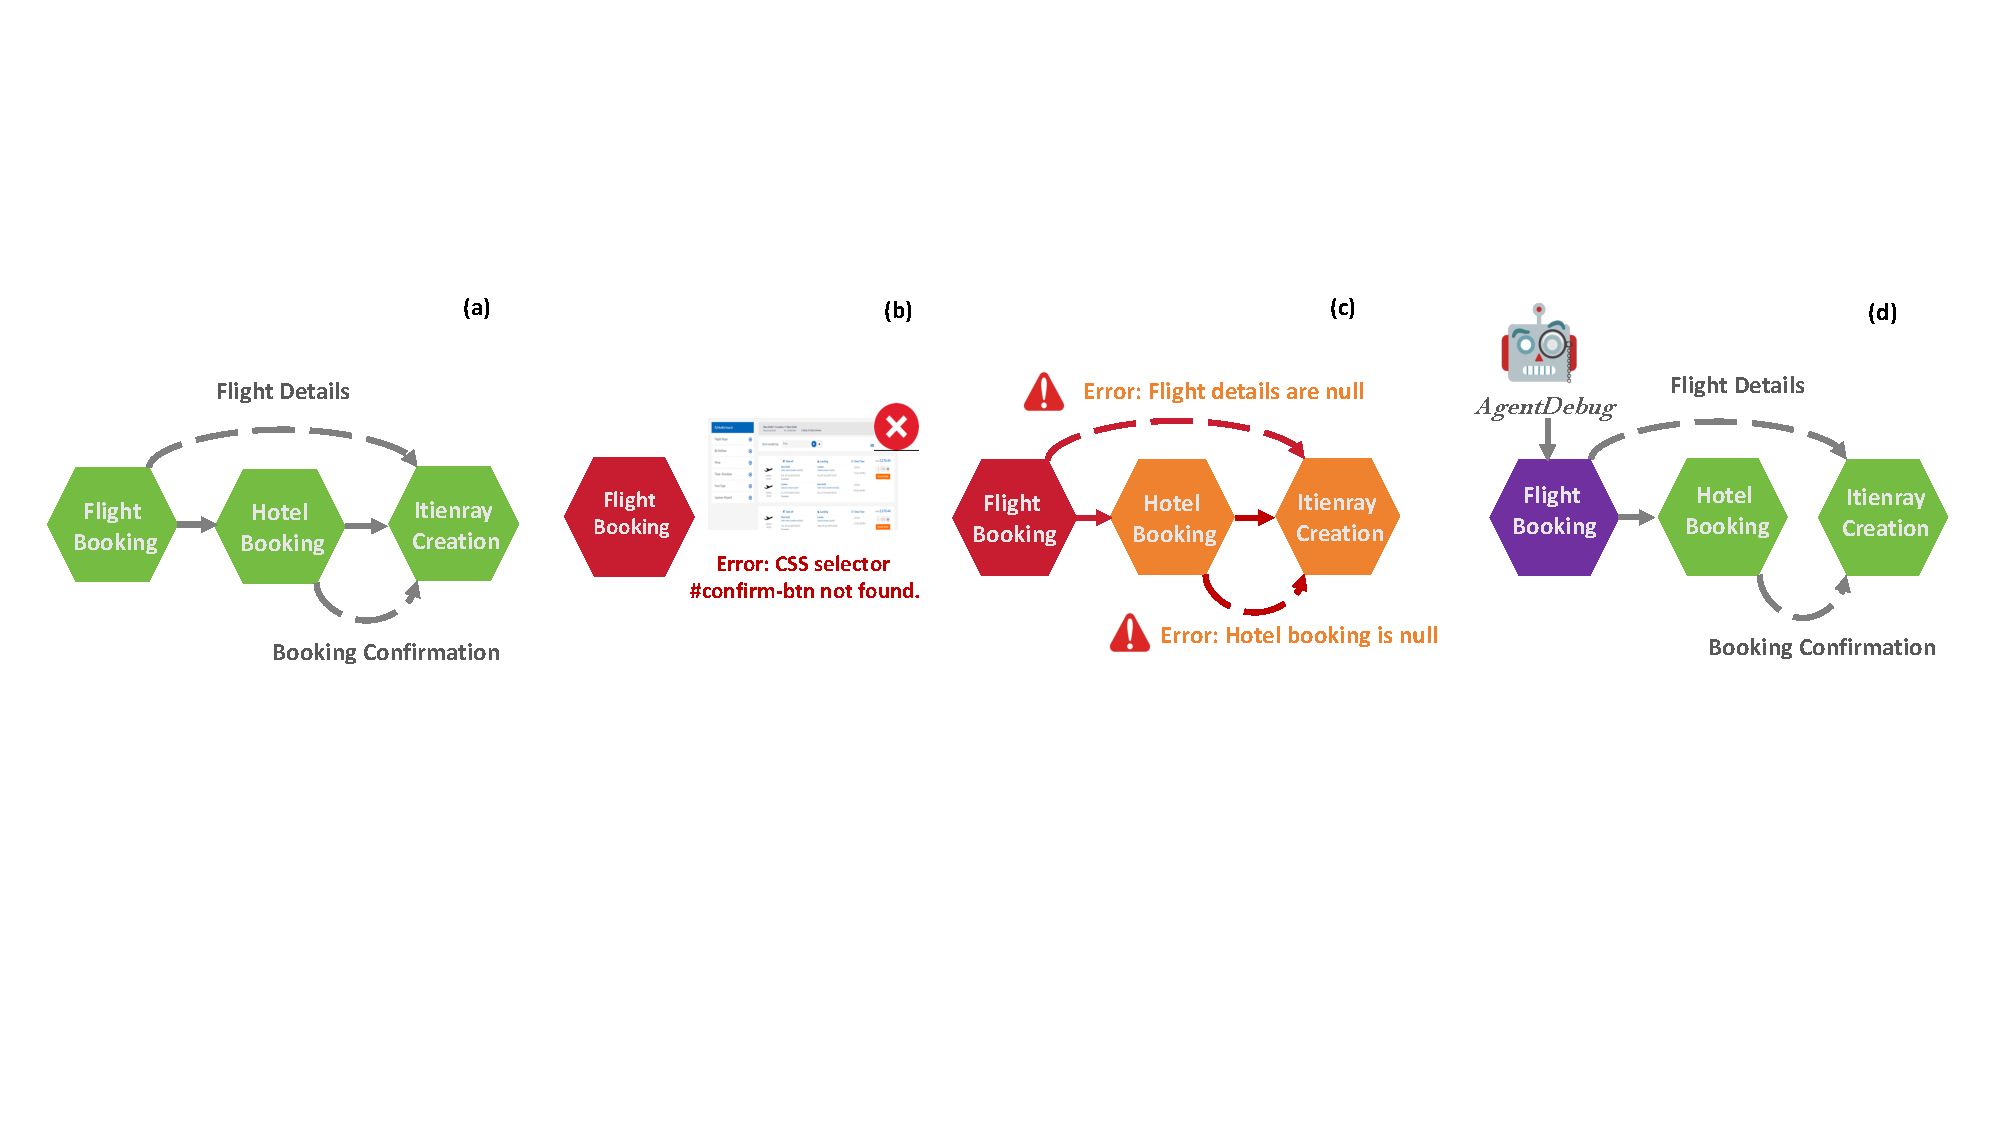
\includegraphics[width=1\linewidth]{figures/teaser.pdf}
    \caption{\textbf{\textit{Motivation for \ModelName{}}}: A single root-cause failure (b) can propagate through subsequent steps (c), compounding errors and leading to task failure. \ModelName{} (d) addresses this bottleneck by tracing failures back to their source and providing actionable feedback that enables agents to evolve into more robust versions.}
    \label{fig:teaser}
    \vspace{-0.2in}
\end{figure}


%%% We identified the key bottleneck- Error Propagation
Our analysis reveals a critical bottleneck in LLM agents: \emph{error propagation}. As illustrated in Figure~\ref{fig:teaser}, a single root-cause failure (b) can cascade into successive errors (c), compounding degradation and leading to task failure. This challenge is especially acute in long-horizon tasks, where early mistakes distort later reasoning and actions, making recovery difficult. These insights motivate our central question: \textit{\textbf{How can LLM agents refine from failures}}?

%%% Prior works 
Recent progress in LLMs agent enhancement has largely centered on expanding the reasoning search space—through chain-of-thought~\citep{wei2023chainofthoughtpromptingelicitsreasoning}, tree-of-thought~\citep{yao2023treeofthoughts}, and graph-of-thought~\citep{besta2023graphofthoughts} approaches—or on incorporating step-level self-reflection \citep{yao2022react, yao2023treeofthoughts, besta2023graphofthoughts}, which allows agents to deliberate more thoroughly and locally revise their actions. While these advances improve flexibility and reasoning depth, they typically treat the trajectory as a sequence of isolated steps rather than as a coherent, interdependent process. 

% In reality, an agent’s trajectory is more akin to a program: it unfolds step by step, with dependencies, state changes, and side effects that accumulate over time. Viewing agents in this way suggests that improving their reliability is not only a modeling challenge but also an engineering one. Just as complex software systems require systematic debugging to trace and correct root-cause errors, agent systems demand principled debugging methodologies to enhance robustness. This perspective motivates us to propose debugging as the foundational mechanism for building more reliable LLM agents.


% summarize
% One of our key observations is that in reality, an agent’s trajectory is more akin to a program: it unfolds step by step, with dependencies, state changes, and side effects that accumulate over time. Viewing agents in this way suggests that improving their reliability is not only a modeling challenge but also an engineering one. Just as complex software systems require systematic debugging to trace and correct root-cause errors, agent systems demand principled debugging methodologies to enhance robustness. This perspective motivates us to propose debugging as the foundational mechanism for building more reliable LLM agents.

To address this challenge, we propose \ModelName{}, a debugging framework that decomposes a trajectory into decision steps, isolates the minimal set of root-cause failures, and provides corrective feedback back to the responsible states or actions. This process not only reduces noise from irrelevant errors but also highlights the key weaknesses that hinder successful task completion. As illustrated in Figure~\ref{fig:teaser} (d), \ModelName{} enables agents to iteratively evolve into more robust versions by learning directly from their failure cases. To rigorously evaluate whether models can detect critical errors and produce actionable feedback, we also construct the \Bench{}. This benchmark grounds the taxonomy in real-world trajectories, offering the first standardized testbed for error detection and debugging.

%%% Experiment summary
We evaluate \ModelName{} on \Bench{}, where it achieves 24\% higher all-correct accuracy (24.3\% vs. 0.3\%) and 17\% higher step accuracy (45.0\% vs. 28.0\%) compared to the strongest baseline. Beyond detection, the targeted feedback generated by \ModelName{} enables agents to iteratively recover from failures, yielding up to 26\% relative improvements in task success across ALFWorld, GAIA, and WebShop. Ablation studies further confirm that focusing on root-cause errors, rather than attempting to fix every surface-level mistake, is key to efficient debugging and meaningful performance gains.
%%%% Contribution
Overall, our contributions are summarized as follows:
\begin{itemize}[leftmargin=1.2em, itemsep=0.1em, topsep=0.25em]
    \item We analyze failed trajectories of LLM agents across diverse benchmarks and show that error propagation—early mistakes cascading into later failures—is the key bottleneck to robustness. From this study, we derive the \AET{}, a unified taxonomy of failure modes spanning planning, tool use, memory, and reflection.
    \item We introduce \Bench{}, the first curated dataset of systematically annotated failures from ALFWorld, GAIA, and WebShop. Each trajectory is labeled with fine-grained error categories and actionable feedback, providing a standardized testbed for studying, benchmarking, and comparing agent debugging methods.
    \item We present \ModelName{}, a debugging framework that identifies critical errors and provides actionable feedback. \ModelName{} achieves high root-cause detection accuracy, exceeding strong baselines by 24\%, and improves task success rates by 26\% across embodied reasoning, web interaction, and decision-making domains.
\end{itemize}


\section{Where do LLM Agents Fail?}
\label{sec:aet_bench}
To lay the foundation for our study of agent failures and debugging, this section introduces two \textit{proposed} components. Section~\ref{sub:aet} presents the \AET{}, a structured framework that organizes recurring failure modes into coherent modules. Section~\ref{sub:bench} then describes the \Bench{}, which grounds this taxonomy in systematically annotated trajectories from multiple environments. 

\begin{figure}[h]
    \centering
    \includegraphics[width=1\linewidth]{iclr2026/figures/aet_bench.pdf}
    \caption{\textbf{Pipeline of proposed \AET{} and \Bench{}}. Failed trajectories are collected, analyzed to develop a taxonomy of errors, and then annotated with root causes and actionable feedback to form the benchmark.}
    \label{fig:aet_bench_construction}
    \vspace{-0.2in}
\end{figure}

\subsection{Agent Failure Analysis}
\label{sub:aet}

To systematically investigate how agents fail, we collected over 500 failed trajectories from ALFWorld, WebShop, and GAIA, and conducted detailed human analyses to uncover recurring patterns. 
This study revealed the following central insight:

\begin{tcolorbox}[colback=berkeleyblue!5!white, colframe=berkeleyblue!100!black, boxrule=0.5mm, left=0.1mm, right=0.1mm, top=0.1mm, bottom=0.1mm]
\textbf{\textit{Key Insight.}} \textit{Error propagation is the primary bottleneck in LLM agent reliability.}  
Early mistakes rarely remain confined; instead, they cascade into subsequent steps, distorting reasoning, compounding misjudgments, and ultimately derailing the entire trajectory.
\end{tcolorbox}

Building on this insight, we introduce the \AET{}, a structured taxonomy that organizes recurring failure modes into five modules. Four capture the core operations of an agent—\textit{memory}, \textit{reflection}, \textit{planning}, and \textit{action}—while a fifth category accounts for \textit{system-level} errors that arise from external tools or infrastructure. This modular view not only enumerates common error types but also clarifies how weaknesses in one stage can cascade into others, enabling a principled approach to tracing and diagnosing failures.

\tcbset{
  colback=white,
  colframe=black!50,
  arc=4pt, % corner radius
  boxrule=0.5pt,
  left=2pt,
  right=2pt,
  top=2pt,
  bottom=2pt
}

\small
\begin{tcolorbox}
\begin{tabular}{>{\bfseries}m{0.18\linewidth} m{0.75\linewidth}}

\rowcolor{orange!10} \textit{Memory} & Errors in recalling or retrieving information (false recall, omission, retrieval failure) that distort subsequent reasoning. \\

\rowcolor{blue!10} \textit{Reflection} & Failures in monitoring progress or interpreting outcomes (progress misassessment, outcome misinterpretation), blocking course correction. \\

\rowcolor{green!10} \textit{Planning} & Logically unsound or infeasible strategies (impossible actions, constraint ignorance, incoherent subgoals) that cascade into missteps. \\

\rowcolor{yellow!15} \textit{Action} & Mistakes in executing operations (malformed outputs, incorrect parameters, missing arguments) that are visible but often mask upstream errors. \\

\rowcolor{red!15} \textit{System-level} & Failures outside reasoning, such as tool crashes, API mismatches, or exceeding step limits, highlighting system robustness issues. \\

\end{tabular}
\end{tcolorbox}

The \AET{} is designed not merely as a catalog of errors but as a causal lens for understanding how failures originate, propagate, and interact across modules. Full definitions are provided in Appendix~\ref{app:aet}.

\subsection{Agent Error Benchmark}
\label{sub:bench}

To rigorously evaluate whether models can detect critical errors and produce actionable feedback, we construct the \Bench{}. This benchmark grounds the taxonomy in real-world trajectories, offering the first standardized testbed for error detection and debugging.

The construction pipeline is shown in Figure~\ref{fig:aet_bench_construction}. We curated 200 representative trajectories: 100 from ALFWorld, 50 from WebShop, and 50 from GAIA. Ten expert annotators—graduate students with prior experience in NLP and LLMs agent research—labeled each trajectory using the \AET{} schema. Annotation proceeded at the decision-step level: every action, reflection, or plan was reviewed, and annotators tagged its error type(s) according to the taxonomy. In addition, they were tasked with identifying the minimal set of root-cause failures that explain the downstream error cascade, rather than exhaustively flagging all surface mistakes. This root-cause focus was emphasized through detailed guidelines and calibration examples, refined iteratively over three rounds of pilot annotation.

To ensure consistency, annotators first completed a training phase with feedback from the authors, followed by independent double-annotation on a shared subset of trajectories. Disagreements were adjudicated collectively, leading to several clarifications in category definitions (e.g., distinguishing “retrieval failure” under memory vs. “constraint ignorance” under planning). The final protocol balanced granularity with reliability, aiming for concise but causally meaningful tags. Inter-annotator agreement, measured using Cohen’s $\kappa$, reached $\kappa = \text{0.55}$ across modules, indicating substantial agreement.

The resulting dataset provides a quantitative view of how agents fail in practice. Figure~\ref{fig:failure_analysis} shows how errors emerge across steps, modules, and error types in the \Bench{}. It shows most failures cluster in mid-trajectory steps (6–15), where early missteps often cascade downstream. Memory and reflection dominate, with retrieval failures, hallucinations, and progress misjudgments leading to flawed planning. Action and system errors occur less frequently but remain critical, as malformed outputs or step-limit exhaustion can immediately terminate trajectories. The complete error type distribution is attached to Appendix \ref{app:failure_analysis}. 


\begin{figure}[htbp]
    \centering
    \includegraphics[width=0.96\linewidth]{iclr2026/figures/Combined_Sankey.pdf}
    \caption{Distribution of failure cases in LLM agents on the \Bench{}}
    \label{fig:failure_analysis}
\end{figure}


Together, \AET{} and \Bench{} provide both the conceptual foundation and the empirical infrastructure for advancing robust LLM agents.


\section{How to Refine LLM Agents from Failures?}
\label{sec:method}

% In low-resource academic setting, collecting a sufficient amount of data to potentially train an debug LLM will be cost prohibitive (est. cost XXX, with human labeling efforts). 
% Instead, we developed an effective LLM workflow via prompt design that is cost efficient.
% Note that our main purpose here is not to develop a SOTA debug LLM, instead, we aim to show that even with low-resource setting, our proposed TAXONOMY is highly effective in building a prompt based debug LLM workflow.


\begin{figure}[htbp]
    \centering
    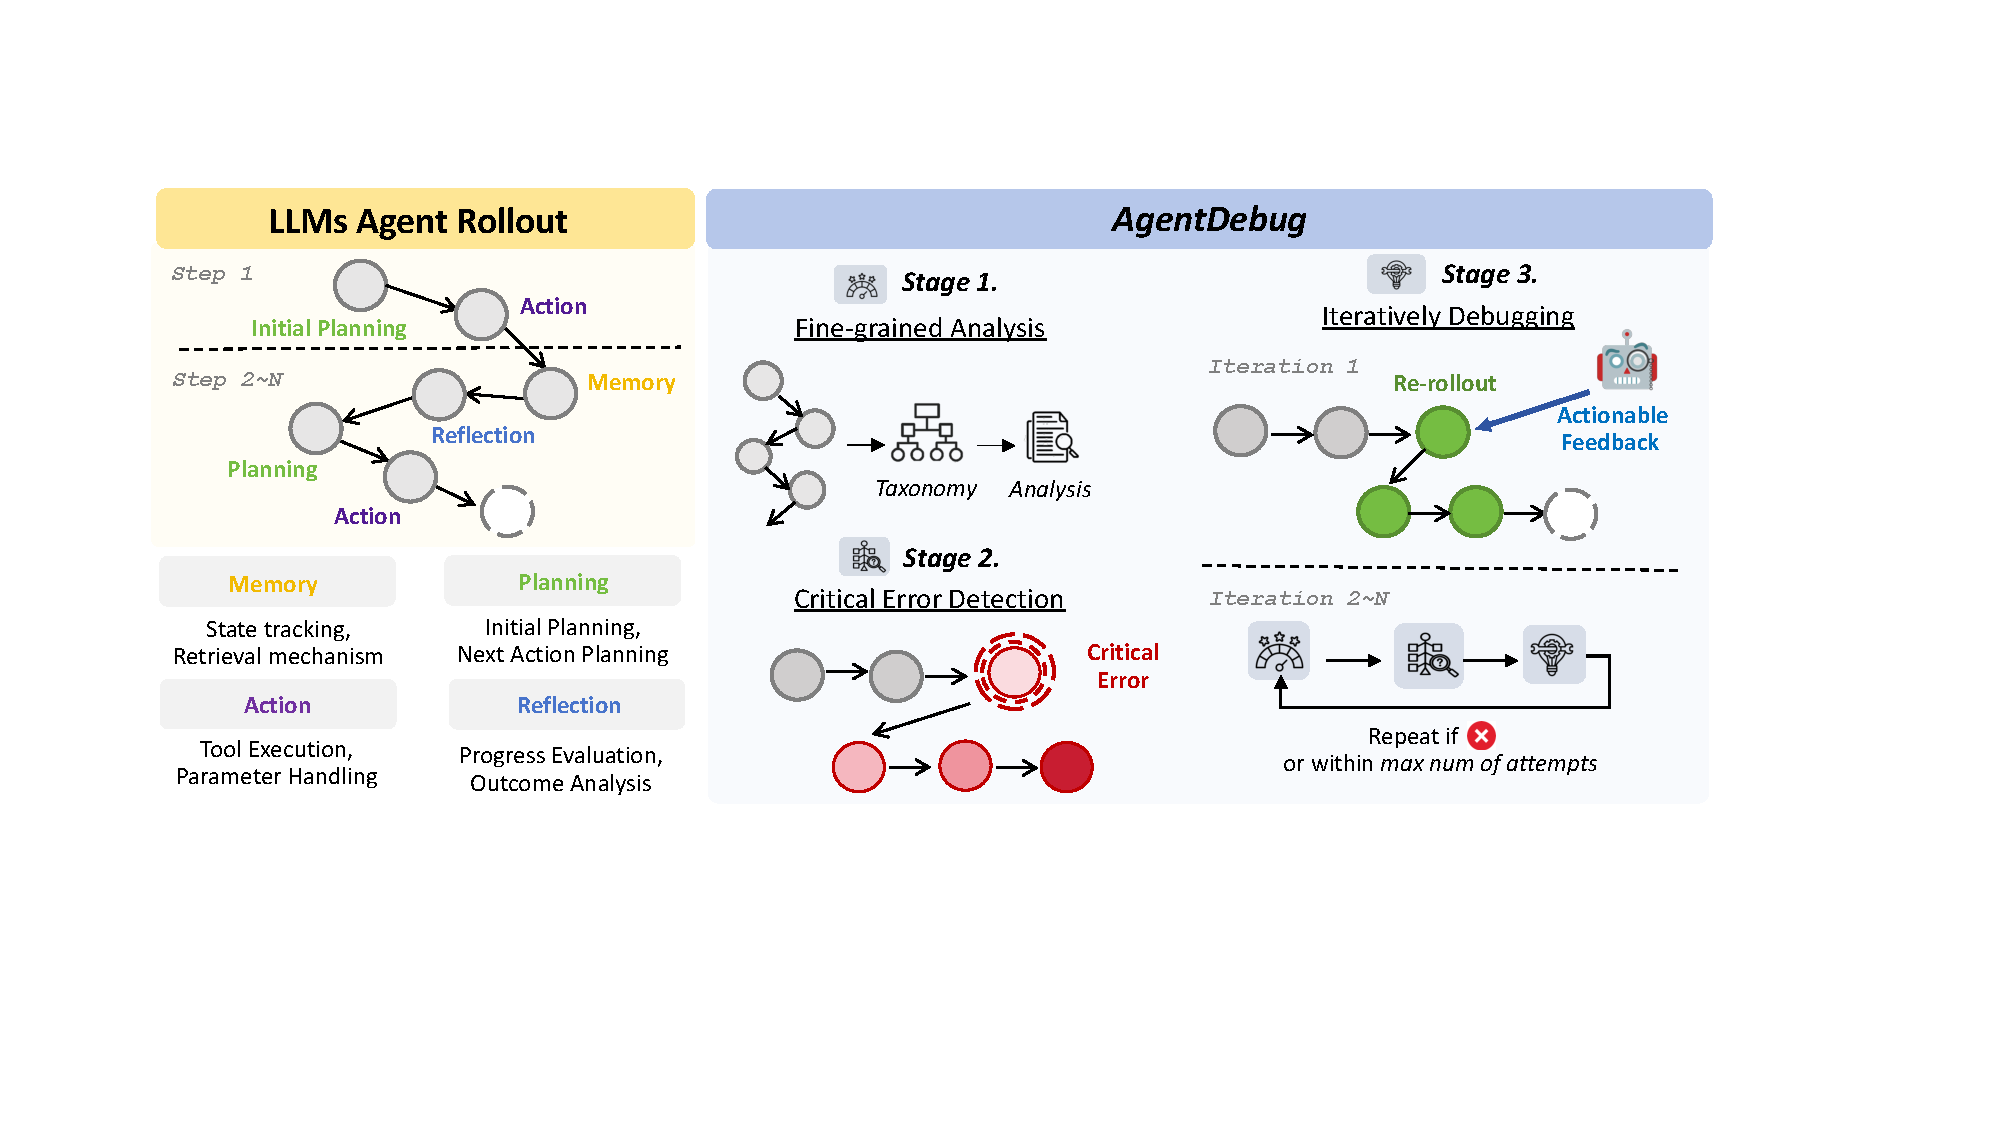
\includegraphics[width=1\linewidth]{figures/method.pdf}
    \caption{\textbf{Overview of \ModelName{}.} (Left) LLM agent rollouts alternate between memory, planning, reflection, and action. (Right) \ModelName{} debugs trajectories in three stages: (1) fine-grained analysis across steps and modules, (2) detection of the critical error that triggers failure, and (3) iterative re-rollouts with actionable feedback to turn failures into successes.}
    \label{fig:method}
\end{figure}


% \begin{algorithm}[h]
% \small
% \DontPrintSemicolon
% \SetAlgoLined
% \LinesNotNumbered
% \KwIn{Trajectory $\tau = \{(s_t, a_t)\}_{t=1}^T$; Error taxonomy $\mathcal{E}_{\text{AET}}$; Max Iterations $I$}
% \KwOut{Corrected trajectory $\tau^*$ \textbf{or} \texttt{Failure}}

% \SetKwFunction{Eval}{Eval}
% \SetKwFunction{MapAET}{MapToAET}
% \SetKwFunction{Correct}{CorrectAction}
% \SetKwFunction{Replace}{ReplaceAction}
% \SetKwFunction{Reroll}{ReRollout}
% \SetKwFunction{GenFB}{GenFeedback}
% \SetKwFunction{UpdFB}{UpdateFeedback}

% \tcc{Stage 1: Fine-grained Analysis with AET}
% \For{$t \gets 1$ \KwTo $T$}{
%   \ForEach{$m \in \{\text{mem}, \text{plan}, \text{refl}, \text{act}\}$}{
%     $e_t^m \gets \MapAET(s_t,a_t,m,\mathcal{E}_{\text{AET}})$ \tcp*{Assign error type per module}
%   }
% }
% \If{\Eval{$\tau$} $=1$}{\Return $\tau$ \tcp*{Trajectory already successful}}

% \tcc{Stage 2: Critical Error Detection via Counterfactuals}
% $t^* \gets \varnothing$ \;
% \For{$t \gets 1$ \KwTo $T$}{
%   $\hat{a}_t \gets \Correct(s_t,a_t,\{e_t^m\}_{m})$ \tcp*{Generate corrected action}
%   $\hat{\tau} \gets \Replace(\tau,t,\hat{a}_t)$ \;
%   \If{\Eval{$\hat{\tau}$} $=1$}{
%     $t^* \gets t$ \tcp*{Earliest correction that removes final failure}
%     \textbf{break}
%   }
% }
% \If{$t^*=\varnothing$}{\Return \texttt{Failure} \tcp*{No critical error found}}

% \tcc{Stage 3: Iterative Debugging with Targeted Feedback}
% $\phi^{(0)} \gets \GenFB(s_{t^*},a_{t^*},\{e_{t^*}^m\}_{m})$ \tcp*{Actionable feedback}
% $\tau^{(0)} \gets \tau$ \;
% \For{$k \gets 1$ \KwTo $I$}{
%   $\tau^{(k)} \gets \Reroll(\tau^{(k-1)}, t^*, \phi^{(k-1)})$ \tcp*{Re-execute from $t^*$ with feedback}
%   \If{\Eval{$\tau^{(k)}$} $=1$}{\Return $\tau^{(k)}$}
%   $\phi^{(k)} \gets \UpdFB(\tau^{(k)}, \phi^{(k-1)})$ \tcp*{Refine guidance if still failing}
% }
% \Return \texttt{Failure} \tcp*{Max Attempts Reached}
% \caption{\ModelName{} Inference Procedure}
% \label{alg:model}
% \end{algorithm}

\begin{algorithm}[h]
\small
\DontPrintSemicolon
\SetAlgoLined
\LinesNotNumbered
\KwIn{Trajectory $\tau = \{(s_t, a_t)\}_{t=1}^T$; Error taxonomy $\mathcal{E}_{\text{AET}}$; Critical-error criterion $\mathcal{C}_{\text{crit}}$; Max Iterations $I$}
\KwOut{Corrected trajectory $\tau^*$ \textbf{or} \texttt{Failure}}

\SetKwFunction{Eval}{Eval}
\SetKwFunction{MapAET}{MapToAET}
\SetKwFunction{Reroll}{ReRollout}
\SetKwFunction{GenFB}{GenFeedback}
\SetKwFunction{UpdFB}{UpdateFeedback}
\SetKwFunction{Detect}{DetectCriticalErrors}

\tcc{Stage 1: Fine-grained Analysis with AET}
\For{$t \gets 1$ \KwTo $T$}{
  \ForEach{$m \in \{\text{mem}, \text{plan}, \text{refl}, \text{act}\}$}{
    $e_t^m \gets \MapAET(s_t,a_t,m,\mathcal{E}_{\text{AET}})$ \tcp*{Assign error type per module}
  }
}
\If{\Eval{$\tau$} $=1$}{\Return $\tau$ \tcp*{Trajectory already successful}}

\tcc{Stage 2: Critical Error Detection via LLM (no rollout/counterfactuals)}
$\mathcal{C} \gets \{\tau,\{e_t^m\}_{t,m},\mathcal{E}_{\text{AET}},\mathcal{C}_{\text{crit}}\}$ \tcp*{Pack analysis, taxonomy \& criterion}
$(\mathcal{T}^*, \mathcal{M}^*, \mathcal{Z}^*, \phi^{(0)}) \gets \Detect(\mathcal{C})$ \tcp*{LLM (fine-grained prompt)}
\If{$\mathcal{T}^*=\varnothing$}{\Return \texttt{Failure} \tcp*{No critical error found}}
$t^* \gets \min(\mathcal{T}^*)$ \tcp*{Earliest critical step}
\tcp{$\mathcal{T}^*$: set of critical steps; $\mathcal{M}^*$: modules per critical step; $\mathcal{Z}^*$: error-types per critical step}

\tcc{Stage 3: Iterative Debugging with Targeted Feedback}
$\tau^{(0)} \gets \tau$ \;
\For{$k \gets 1$ \KwTo $I$}{
  $\tau^{(k)} \gets \Reroll(\tau^{(k-1)}, t^*, \phi^{(k-1)})$ \tcp*{Re-execute from $t^*$ with feedback}
  \If{\Eval{$\tau^{(k)}$} $=1$}{\Return $\tau^{(k)}$}
  $\phi^{(k)} \gets \UpdFB(\tau^{(k)}, \phi^{(k-1)})$ \tcp*{Refine guidance if still failing}
}
\Return \texttt{Failure} \tcp*{Max Iterations Reached}
\caption{\ModelName{} Inference Procedure }
\label{alg:model}
\end{algorithm}


Building on our analysis of agent failures, we aim to develop method that actively refine themselves by learning from mistakes. We first formalize the key modules of an LLM-based agent in Section~\ref{sec:rollout}, and then present our proposed framework, \ModelName{}, in Section~\ref{sec:model}.


\subsection{Key Modules of an LLM Agent}
\label{sec:rollout}
As illustrated in Figure~\ref{fig:method}, we consider an agent that interacts with an environment over a sequence of steps.  
At each step, the agent observes a state and produces an action, forming a trajectory of state–action pairs.  
Each action is generated through four sequential modules: \textbf{Memory}, which recalls relevant past information; \textbf{Reflection}, which evaluates progress and interprets feedback; \textbf{Planning}, which formulates the next strategy; and \textbf{Action}, which executes the low-level operation.  
Errors can occur in any of these modules, and mistakes made early often propagate through later stages, compounding into larger failures.  This modular rollout design not only mirrors the agent’s internal decision process, but also provides a natural structure for human annotators to align errors with specific modules, making the diagnosis of agent failures more transparent and interpretable.  

\subsection{\ModelName{} Framework}
\label{sec:model}
We propose \ModelName{}, a debugging framework that enables single-LLM agents to diagnose and recover from their own failures across diverse environments. As illustrated in Fig.~\ref{fig:method}, \ModelName{} analyzes complete trajectories to (i) assign fine-grained error types to each step and module, (ii) identify the earliest critical error that directly causes the final failure, and (iii) provide actionable feedback to guide re-rollouts. The central intuition is that correcting a single root-cause mistake can often flip an otherwise failing trajectory into a successful one.

As presented in Algorithm~\ref{alg:model}, the inference procedure of \ModelName{} consists of three stages:

\paragraph{Stage 1: Fine-grained Analysis with \AET{}.}  
For each step in the trajectory, we analyze all four modules—memory, reflection, planning, and action.  
Each module is mapped to an \AET{} error type, grounding the analysis in interpretable categories such as “constraint ignorance” or “format error.”  
This produces a structured, module-level error profile for the trajectory.  

\paragraph{Stage 2: Critical Error Detection via Counterfactuals.}  
If the trajectory is already successful, no debugging is required.  
Otherwise, we perform counterfactual testing step by step: at each point, we substitute a corrected action and test whether the rollout would succeed.  
The \emph{critical error} is defined as the earliest step whose correction directly prevents the final failure.  
Unlike superficial mistakes or errors that are later corrected, the critical error is the root cause that truly determines whether the overall trajectory succeeds or fails—capturing both \emph{when} and \emph{why} the agent goes irreversibly off track.  

\paragraph{Stage 3: Iterative Debugging with Targeted Feedback.}  
Once the critical error is identified, the system generates feedback that specifies the error type and provides actionable guidance for refining subsequent actions and plans.  
The agent then re-executes (re-rolls out) the trajectory under this feedback. If the rollout still fails, the feedback is refined with more specific guidance, and the process repeats up to a fixed budget of attempts.  
Grounded in the \AET{} taxonomy, the feedback is both targeted and forward-looking—resolving the root cause while shaping how the agent approaches future steps.  





\section{Experiments and Results}
\label{sec:experiment}
\subsection{Critical Error Detection}
\label{subsec:rootcause}

\noindent{\textbf{Dataset.}}
We evaluate critical error localization on \Bench{} (Sec.~\ref{sub:bench}), which consists of 200 annotated failure trajectories.  
These trajectories are drawn from three representative benchmarks: \textbf{ALFWorld} \citep{shridhar2020alfworld}, \textbf{GAIA} \citep{mialon2023gaia}, and \textbf{WebShop} \citep{yao2022webshop}.  

\noindent{\textbf{Baselines.}}
We compare against three strategies: (1) \textbf{Direct Prompting}, which queries the LLM directly for error localization without any structured search; (2) \textbf{Brute Force}, which examines steps sequentially from $t{=}1$ to $T$, substituting a corrected action at each step and stopping once the rollout succeeds, thereby identifying the earliest critical step; and (3) \textbf{Binary Search}, which applies a divide-and-conquer procedure by probing the midpoint of the trajectory and recursively halving the search space until the critical step is isolated.  

\noindent{\textbf{Implementation.}}
We use GPT-4.1 as the base model, with the temperature set to 0 for deterministic outputs. The full prompt template is provided in the Appendix \ref{app:prompt}. 

\noindent{\textbf{Evaluation Metic.}} We evaluate critical error detection at multiple granularities, capturing both partial and complete localization ability. Specifically, we measure \textbf{Step} accuracy, the ability to identify the exact step where the first critical error occurs; %\textbf{Error Type} accuracy, the assignment of the correct fine-grained \AET{} label (e.g., constraint ignorance, format error); 
\textbf{Step+Module} accuracy, the joint prediction of both the correct step and its module; and \textbf{All Correct} (Step+Module+Error Type), a strict metric requiring the exact step, module, and error type to all be correctly identified.


\noindent{\textbf{Experiment Results}}  
Table~\ref{tab:exp1} shows that \ModelName{} consistently surpasses baselines across datasets and metrics. On average, \ModelName{} is 24\% more accurate in the All-Correct metric (24.3\% vs.\ 0.3\%) and improves Step accuracy by 61\% (45.0\% vs.\ 28.0\%). The gains are especially pronounced on GAIA, where Step accuracy nearly doubles (58.0\% vs.\ 30.0\%) and All-Correct triples (38.0\% vs.\ 12.0\%).

\begin{table}[hbtp]
\centering
\definecolor{GreenDark}{HTML}{34A853}
\definecolor{GreenLight}{HTML}{E6F4EA}
% 2. WebShop - 橙色系
\definecolor{OrangeDark}{HTML}{FBBC04}
\definecolor{OrangeLight}{HTML}{FEF8E7}
% 3. GAIA - 紫色系
\definecolor{PurpleDark}{HTML}{A142F4}
\definecolor{PurpleLight}{HTML}{F3E8FD}
% 4. Average - 粉色系
\definecolor{PinkDark}{HTML}{FF6D70}
\definecolor{PinkLight}{HTML}{FFEEEE}

\setlength{\tabcolsep}{6pt} % 调整列间距
\renewcommand{\arraystretch}{1.2} % 调整行高

\resizebox{\linewidth}{!}{\begin{tabular}{l ccc ccc ccc ccc}
\toprule
& \multicolumn{3}{c}{\cellcolor{GreenDark}\color{white}\textbf{ALFWorld}}
& \multicolumn{3}{c}{\cellcolor{OrangeDark}\color{white}\textbf{WebShop}}
& \multicolumn{3}{c}{\cellcolor{PurpleDark}\color{white}\textbf{GAIA}}
& \multicolumn{3}{c}{\cellcolor{PinkDark}\color{white}\textbf{Average}} \\

\cmidrule(lr){2-4} \cmidrule(lr){5-7} \cmidrule(lr){8-10} \cmidrule(lr){11-13}

% --- 表头第二行：S, S+M, ALL ---
\textbf{Method}
& \cellcolor{GreenDark}\color{white}S & \cellcolor{GreenDark}\color{white}S+M & \cellcolor{GreenDark}\color{white}ALL
& \cellcolor{OrangeDark}\color{white}S & \cellcolor{OrangeDark}\color{white}S+M & \cellcolor{OrangeDark}\color{white}ALL
& \cellcolor{PurpleDark}\color{white}S & \cellcolor{PurpleDark}\color{white}S+M & \cellcolor{PurpleDark}\color{white}ALL
& \cellcolor{PinkDark}\color{white}S & \cellcolor{PinkDark}\color{white}S+M & \cellcolor{PinkDark}\color{white}ALL \\
\midrule

% --- 数据行：Baseline 方法 ---
Direct Prompting
& \cellcolor{GreenLight}28.0\% & \cellcolor{GreenLight}14.0\% & \cellcolor{GreenLight}1.0\%
& \cellcolor{OrangeLight}30.0\% & \cellcolor{OrangeLight}6.0\% & \cellcolor{OrangeLight}0.0\%
& \cellcolor{PurpleLight}26.0\% & \cellcolor{PurpleLight}10.0\% & \cellcolor{PurpleLight}0.0\%
& \cellcolor{PinkLight}28.0\% & \cellcolor{PinkLight}10.0\% & \cellcolor{PinkLight}0.3\% \\

Brute Force
& \cellcolor{GreenLight}10.0\% & \cellcolor{GreenLight}5.0\% & \cellcolor{GreenLight}0.0\%
& \cellcolor{OrangeLight}8.0\% & \cellcolor{OrangeLight}0.0\% & \cellcolor{OrangeLight}0.0\%
& \cellcolor{PurpleLight}18.0\% & \cellcolor{PurpleLight}8.0\% & \cellcolor{PurpleLight}0.0\%
& \cellcolor{PinkLight}12.0\% & \cellcolor{PinkLight}4.3\% & \cellcolor{PinkLight}0.0\% \\

Binary Search
& \cellcolor{GreenLight}20.0\% & \cellcolor{GreenLight}6.0\% & \cellcolor{GreenLight}1.0\%
& \cellcolor{OrangeLight}14.0\% & \cellcolor{OrangeLight}8.0\% & \cellcolor{OrangeLight}0.0\%
& \cellcolor{PurpleLight}22.0\% & \cellcolor{PurpleLight}10.0\% & \cellcolor{PurpleLight}0.0\%
& \cellcolor{PinkLight}18.7\% & \cellcolor{PinkLight}8.0\% & \cellcolor{PinkLight}0.3\% \\
\midrule

\textbf{\ModelName{}}
& \cellcolor{GreenLight}\textbf{35.0\%} & \cellcolor{GreenLight}\textbf{28.0\%} & \cellcolor{GreenLight}\textbf{21.0\%}
& \cellcolor{OrangeLight}\textbf{42.0\%} & \cellcolor{OrangeLight}\textbf{22.0\%} & \cellcolor{OrangeLight}\textbf{14.0\%}
& \cellcolor{PurpleLight}\textbf{58.0\%} & \cellcolor{PurpleLight}\textbf{44.0\%} & \cellcolor{PurpleLight}\textbf{38.0\%}
& \cellcolor{PinkLight}\textbf{45.0\%} & \cellcolor{PinkLight}\textbf{31.3\%} & \cellcolor{PinkLight}\textbf{24.3\%} \\

\bottomrule
\end{tabular}}
\caption{Comparison of methods across three environments (ALFWorld, WebShop, GAIA) and their average performance. Our method consistently outperforms baselines in all settings. Metrics shown are Step Exact (S), Step+Module (S+M), and All Correct (ALL).}
\label{tab:exp1}
\end{table}




% \begin{table}[htbp]
% \centering
% \small
% \renewcommand{\arraystretch}{1.0} % Adjust row spacing
% \setlength{\tabcolsep}{6pt} % Adjust column spacing
% \resizebox{\linewidth}{!}{
% \begin{tabular}{
%     l
%     |>{\columncolor{Color1}}c
%     |>{\columncolor{Color2}}c
%     |>{\columncolor{Color3}}c
%     |>{\columncolor{Color4}}c
%     |>{\columncolor{Color5}}c
%     |>{\columncolor{Color6}}c
% }
% \toprule
% \textbf{Method} & \textbf{Step} & \textbf{Step ($\pm$3)} & \textbf{Module} & \textbf{Error Type} & \textbf{Step+Module} & \textbf{All Correct} \\
% \midrule
% Direct Prompting & 12.5 & 65.0 & 50.0 & 25.0 & 12.5 & 7.5 \\
% Brute Force      & 10.0 & 55.0 & 32.5 & 15.0 & 2.5  & 2.5 \\
% Binary Search    & 5.0  & 25.0 & 15.0 & 10.0 & 0.0  & 0.0 \\
% \midrule
% Ours             & \textbf{50.0} & \textbf{85.0} & \textbf{65.0} & \textbf{50.0} & \textbf{45.0} & \textbf{42.5} \\
% \bottomrule
% \end{tabular}
% }
% \caption{Critical Error Detection experiment results on \Bench{}.}
% \label{tab:detection}
% \end{table}





\subsection{Downstream Debugging on Single-Agent Benchmarks}
\label{subsec:downstream}

We next evaluate whether improved error detection leads to higher task success, testing if localizing root-cause failures enables agents to recover more effectively than baselines.

\noindent\textbf{Datasets.}  
Follow the previous experiment setting, we choose the evaluation data from three widely used single-agent benchmarks that cover complementary domains of reasoning and interaction: \textbf{ALFWorld} \citep{shridhar2020alfworld}, \textbf{GAIA} \citep{mialon2023gaia}, \textbf{WebShop} \citep{yao2022webshop}.

\noindent\textbf{Baselines.}  
We compare \textsc{AgentDebug} against several strong approaches. The first is Self-Refine, where the agent iteratively revises its outputs without explicit causal diagnosis of errors. The second is a Vanilla Debugger, which applies naive post-hoc corrections to failed trajectories without identifying the critical error taxonomy. Finally, we include strong test-time scaling baselines: Tree-of-Thought (ToT) and Best-of-$N$.  To ensure fairness, the max number of attempts of all baselines is matched to \textsc{AgentDebug} by total token usage, so any observed gains can be attributed to targeted error recovery rather than higher resource allocation.  

\noindent\textbf{Implementation.}  
We implement \textsc{AgentDebug} with up to $N=5$ re-rollouts, each beginning precisely at the identified critical step. This design enables the agent to explore alternative continuations directly from the point of failure rather than restarting from the beginning of the trajectory, thereby concentrating computational effort where it is most impactful. For backbone models of LLMs Agent, we evaluate across three representative systems of varying scales and architectures: GPT-4o-mini, Qwen3-8B, and Qwen3-Next-80B. 

\noindent\textbf{Experiment Results.} Figure~\ref{fig:experiment_4_2_1} reports the performance of \ModelName{} on the ALFWorld benchmark across three backbone LLM agents. On GPT-4o-mini, \ModelName{} boosts success from 21 (first attempt) to 55; on Qwen3-8B, from 48 to 74; and on Qwen3-Next-80B, from 60 to 84. These results show that \ModelName{} consistently outperforms all baselines and can effectively help LLM agents improve regardless of the backbone model, with especially large relative gains for smaller models. 


\begin{figure}[htbp]
    \centering
    \includegraphics[width=1\linewidth]{iclr2026/figures/agent_tts_alfworld_comparison_tight.pdf}
    \caption{Downstream debugging performance on ALFWorld. Results are shown across three backbone models (GPT-4o-mini, Qwen3-8B, Qwen3-Next-80B) and differnt methods. \ModelName{} consistently outperforms strong baselines.}
    \label{fig:experiment_4_2_1}
\end{figure}

\begin{wrapfigure}{r}{0.40\textwidth}
    \vspace{-6pt} % tighten space above (tweak as needed)
    \centering
    \includegraphics[width=\linewidth]{iclr2026/figures/horizontal_comparison.pdf}
    \caption{Performance improvements comparison.}
    \label{fig:experiment_4_2_2}
    \vspace{-6pt} % tighten space below (tweak as needed)
\end{wrapfigure}


To further assess the generalizability of \ModelName{}, we move beyond ALFWorld and extend our evaluation to two additional benchmarks that stress complementary dimensions of agent reasoning: GAIA, which requires integrating open-domain knowledge and web-based tool use, and WebShop, which evaluates agents in a realistic e-commerce setting with structured constraints and transactional goals. Together, these benchmarks provide a diverse testbed spanning embodied interaction, knowledge-grounded reasoning, and goal-directed web navigation. Given the higher computational demands of these settings, we focus on comparing \ModelName{} against the two strongest baselines from our earlier experiments—Self-Refine and Best-of-$N$—which represent state-of-the-art approaches to iterative refinement and test-time scaling, respectively. The results, shown in Figure~\ref{fig:experiment_4_2_2}, demonstrate that \ModelName{} consistently delivers the largest gains across all three benchmarks. In particular, it achieves improvements of up to 26\% on ALFWorld and strong average performance on GAIA and WebShop, underscoring its robustness across diverse environments and confirming that targeted error detection and correction can outperform broader but less focused strategies such as scaling rollouts or unguided self-revision.


\begin{tcolorbox}[colback=californiagold!5!white, colframe=californiagold!100!black, boxrule=0.5mm, left=0.1mm, right=0.1mm, top=0.1mm, bottom=0.1mm]
\textbf{\textit{Findings}.} \ModelName{} consistently outperforms strong baselines in both error detection and downstream task success. Its ability to precisely localize root-cause failures (50.0\% step accuracy and 42.5\% all-correct accuracy) translates into substantial improvements in task performance, achieving up to 26\% relative gains across ALFWorld, GAIA, and WebShop. 
%These results highlight the effectiveness of principled debugging as a pathway toward more robust LLM agents.
\end{tcolorbox}


% \begin{tcolorbox}[colback=berkeleyblue!5!white, colframe=berkeleyblue!100!black, boxrule=0.5mm, left=0.1mm, right=0.1mm, top=0.1mm, bottom=0.1mm]
% \textbf{Takeaway.} ...
% \end{tcolorbox}



\section{Analysis and Discussion}
\label{sec:discussion}
\subsection{Ablation Study}

% 1. Ablation on the debug step over three models on alfoworld test 100, gpt-4o-mini, qwen3-8b, qwen3-next-80b

% 2. Ablations on the different dection models

% 3. ablations on different rollout method:REACT REFLEXION, ACT ONLY, WITH MEMORY


To better understand the contribution of each component in our framework, we conduct a series of ablation studies. Specifically, we analyze the following factors.

\noindent{\textbf{Max Number of Attempts Allowed.}}  
We vary the maximum number of attempts of \ModelName{} with different base models— GPT-4o-mini, Qwen3-8B, and Qwen3-Next-80B—to examine how sensitive performance is to the chosen point of intervention. Results in Figure~\ref{fig:alfworld_success_rates} show that additional attempts yield consistent gains across all backbones, with especially pronounced improvements on smaller models such as GPT-4o-mini. This highlights the value of targeted re-rollouts in boosting task success.

\noindent{\textbf{\ModelName{} Base Models.}}  
We replace the base model of \ModelName{} with several alternatives to assess their impact on error localization and downstream success. As shown in Figure~\ref{tab:ablation_detector}, GPT-4.1 substantially outperforms other models, achieving 42\% step accuracy and 32\% strict all-correct accuracy. Competing base models such as Llama-3.3-70B, GPT-4o-mini, and Qwen3-Next-80B perform markedly worse.

\noindent{\textbf{Rollout Strategies.}}  
We compare several rollout paradigms—ReAct, Reflection, Act-only, and Memory+ReAct—against our proposed \textbf{Modular} strategy on Alfworld under the zero-shot setting. As shown in Table~\ref{tab:ablation_rollout}, \ModelName{}’s Modular rollout achieves the highest score (0.38), outperforming both reasoning-only and memory-augmented baselines. This result highlights the effectiveness of structured modularization is more reliably than alternative rollout designs.


\begin{figure}[htbp]
\centering

% --- Column 1: Plot ---
\begin{subfigure}{0.55\linewidth}
    \centering
    \includegraphics[width=\linewidth]{iclr2026/figures/task_success_rates_qwen_grouped.pdf}
    \caption{Success rates on Alfworld across five attempts.}
    \label{fig:alfworld_success_rates}
\end{subfigure}%
\hfill
% --- Column 2: Stacked Tables ---
\begin{subfigure}{0.45\linewidth}
    \centering
    
    % --- Subfigure B: Detector Table ---
    \begin{subfigure}{\linewidth}
        \centering
        \scriptsize
        \begin{tabular}{lcccc}
        \toprule
        \textbf{Base Model} & \textbf{Step} & \textbf{Error} & \textbf{Step+M} & \textbf{All} \\
        \midrule
        Llama-3.3-70B    & 16.0 & 16.0 & 6.0 & 2.0 \\
        GPT-4o-mini  & 14.0 & 10.0 & 4.0 & 2.0 \\
        Qwen3-Next-80B    &  4.0 & 14.0 & 2.0 & 2.0 \\
        \rowcolor{yellow!20}\textbf{GPT-4.1} & \textbf{42.0} & \textbf{44.0} & \textbf{32.0} & \textbf{32.0} \\
        \bottomrule
        \end{tabular}
        \caption{Base Model Performance Comparison.}
        \label{tab:ablation_detector}
    \end{subfigure}
    
    \vspace{0.5cm}
    
    % --- Subfigure C: Rollout Table (wider) ---
    \begin{subfigure}{1.1\linewidth} % make table C wider
        \centering
        \scriptsize
        \begin{tabular}{lc}
        \toprule
        \textbf{Rollout Strategy} & \textbf{Success Rate} \\
        \midrule
        Memory+ReAct & 0.34 \\
        Reflection   & 0.32 \\
        ReAct        & 0.26 \\
        Act Only     & 0.10 \\
        \rowcolor{yellow!20}\textbf{Modular} & \textbf{0.38} \\
        \bottomrule
        \end{tabular}

        \caption{Rollout Strategy Comparison.}
        \label{tab:ablation_rollout}
    \end{subfigure}
    
\end{subfigure}


\caption{Ablation study results. (a) Success rates on Alfworld, (b) comparison of detector models, and (c) rollout strategy analysis.}
\label{fig:ablation_combined}
\vspace{-0.1in}
\end{figure}

\subsection{Error Propagation}
\label{subsec:error_propoagate}

% Discussion over the error propagation, graphics and statistics
% some statistics by human and llm judge

% how often it cause the cascading effect(not always)

% how length it will cause the cascading effect

% which module and steps range cause the most of 

% some take away to prevent 

A key challenge in building robust LLM agents lies in understanding how small mistakes evolve into large-scale failures. Our analysis examines the phenomenon of error propagation—cases where an early misstep triggers a cascading effect that spreads throughout the trajectory. As shown in Figure \ref{fig:error_propagation},  early-stage mistakes cascade through later steps across tasks. The outlined cells indicate the first critical error in each trajectory, while progressively darker red shading reflects the compounding severity and persistence of errors over subsequent steps. This illustrates how initial failures frequently propagate forward, amplifying downstream task breakdowns.

\begin{figure}[ht]
    \centering
    \vspace{-8mm}
    \includegraphics[width=1\linewidth]{iclr2026/figures/grid_10x30_levels.pdf}
    \caption{\textbf{\textit{Illustration of Error Propagation}}: Darker shading indicating compounding failures and highlighting how initial mistakes amplify downstream breakdowns.}
    \vspace{-0.20in}
    \label{fig:error_propagation}
\end{figure}

Moreover, the likelihood and length of cascades vary significantly across modules. Memory and reflection errors are the most common sources of propagation, typically arising in early or mid-trajectory steps (around steps 5–15). Once an agent misremembers a fact or misjudges its progress, subsequent planning becomes systematically distorted, leading to repeated cycles of flawed action selection. Planning errors also contribute heavily, with constraint ignorance or infeasible strategies compounding as the agent attempts to execute them. By contrast, action-level errors are more visible and sometimes recoverable, though malformed outputs or missing parameters can still derail execution. System-level issues such as tool crashes or step-limit exhaustion act as immediate termination points rather than cascades.

These findings highlight two important takeaways for designing more reliable agents. First, \textbf{early detection and correction are critical}, since once cascades begin, they are difficult to reverse. Second, mechanisms that strengthen memory retrieval and reflection—such as external memory, progress tracking, or verification prompts—can substantially reduce the risk of propagation.




% \subsection{Case Study}
% sucessful debug case and how it can evolve through 

% one more specific error propagation case

% Statistics on the error types and steps distribution on benchmarks




\section{Related Work}
\label{sec:related_works}

\paragraph{LLM-based Agentic Systems.}
Recent advances in LLM-based agents have demonstrated that combining planning, tool use, memory, and self-reflection can substantially improve performance on complex, multi-step tasks. The reasoning-acting paradigm, pioneered by ReAct \citep{yao2022react}, interleaves chain-of-thought reasoning with grounded environment actions. Test-time search methods such as Tree-of-Thoughts \citep{yao2023treeofthoughts} and Graph-of-Thoughts \citep{besta2023graphofthoughts} further expand the deliberation space through structured exploration. These systems are strengthened by external tool integration, ranging from self-supervised tool selection in Toolformer \citep{schick2023toolformer} to comprehensive tool ecosystems in ToolLLM \citep{qin2023toolllm}, as well as persistent memory mechanisms that maintain context across long horizons \citep{packer2023memgpt}. A critical aspect of robustness is the ability to reflect and self-correct: Reflexion \citep{shinn2023reflexion} introduces verbal self-reflection to revise future actions, while subsequent work explores richer feedback modalities and meta-cognitive strategies for deciding when to reflect versus act. Despite recent advances, the community still lacks a unified view of how agent components interact and fail. \ModelName{} fills this gap with a debugging layer that traces root causes across the plan–act–observe loop, detects failures from tool-use to memory, and generates corrective feedback that enables agents to improve through their mistakes.
\vspace{-0.1in}
\paragraph{Failure Analyses (Single- and Multi-Agent).}
Systematic failure analyses are emerging to quantify where agents break and how errors propagate. In multi-agent settings, recent works examine collaboration and competition dynamics~\citep{zhu2025multiagentbench}, role specialization, and emergent failure modes such as coordination collapse and dialogue drift \citep{cemri2025why,zhang2025which,zhu2025multiagentbench,hyun2025crewwildfire,tran2025multiagent}. For single-agent systems, analyses have highlighted planning brittleness, grounding and tool-use errors, and hallucination-induced cascades \citep{ji2024testing,sung2025verila,ning2024defining}. Compared to these studies, we focus on actionable debugging: moving from descriptive taxonomies to a two-stage detector that both identifies and helps fix root causes.
\vspace{-0.1in}
\paragraph{Test-Time Scaling for Agents.}
Scaling test-time compute improves reasoning and success rates by allocating more deliberation to challenging instances. In agents, this includes tree/graph search in thought space \citep{yao2023treeofthoughts,besta2023graphofthoughts}, best-of-$N$ sampling with self-consistency, and test-time compute scaling strategies \cite{li2025metal}. Our experiments position \ModelName{} orthogonally to compute scaling: even at fixed compute, targeted debugging recovers substantial performance, and when combined with scaling, it channels extra compute to the right failure points.

\vspace{-0.1in}

\section{Conclusion}
\label{sec:conclusion}
In summary, our work identifies error propagation as the central bottleneck to building robust LLM agents and introduces \AET{}, \Bench{}, and \ModelName{} as principled solutions. By tracing and correcting root-cause failures, \ModelName{} achieves substantial performance gains and establishes debugging as a foundation for agents that can continuously learn and evolve from their mistakes. While our work has limitations (see Appendix~\ref{app:limitation}), it paves the way toward more reliable and adaptive LLMs Agent.


\section*{Ethical Statement}
This work focuses on analyzing and improving the robustness of LLM-based agents. Our study does not involve human subjects, sensitive personal data, or information that could directly identify individuals. All experiments were conducted on publicly available benchmarks (ALFWorld, GAIA, and WebShop) under their respective licenses. While our findings aim to advance reliability and transparency in LLM agents, we acknowledge that more capable debugging frameworks could potentially be misused to strengthen harmful or malicious agents. We encourage responsible use of our methods, with applications limited to domains that respect safety, fairness, and accountability.

\section*{Acknowledgment}
We thank the OpenManus team, including Chenglin Wu, Jiayi Zhang, Xinbing Liang, and Jingyu Xiang, for their valuable assistance in the discussion and for providing some resources.


% \section*{LLM Use Statement}
% LLM were used in two ways during this work. First, LLMs served as the backbone agents evaluated in our experiments (e.g., GPT-4.1, GPT-4o-mini, Qwen3-8B, Qwen3-Next-80B, Llama 3.1-70B). Second, we used LLMs to assist with writing tasks such as grammar error checking, and formatting, but all conceptual contributions, experimental design, and analyses were performed by the authors. 


% \subsubsection*{Author Contributions}
% If you'd like to, you may include  a section for author contributions as is done
% in many journals. This is optional and at the discretion of the authors.

% \subsubsection*{Acknowledgments}
% Use unnumbered third level headings for the acknowledgments. All
% acknowledgments, including those to funding agencies, go at the end of the paper.


\bibliography{iclr2026_conference}
\bibliographystyle{iclr2026_conference}

\clearpage
\appendix
\section{Appendix}
% todo: taxnomy graph
% examples of the agentdebug graph
% examples of the dataset over different error types
% example of the real error propagation case

% example of the rollout with 4 modules

\subsection{Limitation}
\label{app:limitation}
Our work is not without limitations. First, while \Bench{} covers three representative benchmarks (ALFWorld, GAIA, and WebShop), it remains limited in scale and domain diversity; extending to multimodal environments, longer-horizon tasks, or safety-critical applications (e.g., healthcare, finance) is an important direction for future work. Second, collecting sufficient data to train a dedicated debugging model would be prohibitively expensive in low-resource academic settings, given the costs of large-scale human annotation. To mitigate this, we instead designed a cost-efficient workflow that leverages prompt engineering with existing LLMs, though this approach may still fall short of the performance achievable with a fully trained, specialized model.


\clearpage
\subsection{\AET{}}
\label{app:aet}
\begin{figure}[htbp]
    \centering
    \includegraphics[width=0.7\linewidth]{iclr2026/figures/agent_error_sunburst.pdf}
    \caption{\textbf{Error Taxonomy across all modules}: The hierarchical taxonomy organizes agent errors into five core modules—\emph{Planning}, \emph{Action}, \emph{Reflection}, \emph{Memory}, and \emph{System}. Each outer ring category specifies representative error types, such as constraint ignorance or inefficient planning (Planning), parameter or format errors (Action), causal misattribution or outcome misinterpretation (Reflection), oversimplification or false memory (Memory), and tool execution or environment errors (System). This taxonomy provides a holistic view of where and how failures emerge within modular LLM agents.}

    \label{fig:error_taxnomy}
\end{figure}
\input{iclr2026/appendix/aet}

\clearpage

\subsection{AgentDebug Example}
\begin{figure}[htbp]
    \centering
    \includegraphics[width=1\linewidth]{iclr2026/figures/AgentDebug_example.pdf}
    \caption{\textbf{AgentDebug example on ALFWorld:} Comparison between a normal agent (left) and our method AgentDebug (right). AgentDebug successfully pinpoints the critical error in the \emph{Plan} module (inefficient cabinet-only search) and provides actionable feedback (expand to countertops/tables). This guidance allows the agent to recover from failure and complete the task successfully.}


    \label{fig:error_taxnomy}
\end{figure}
\clearpage
\subsection{Failure Analysis Across Representative LLMs Agent Benchmarks}
\label{app:failure_analysis}

\begin{figure}[htbp]
    \centering
    \includegraphics[width=0.8\linewidth]{iclr2026/figures/AlfWorld_Sankey.pdf}
    \caption{Distribution of failure cases in LLM agents on the Alfworld benchmark.}
    \label{fig:failure_analysis}
\end{figure}

\begin{figure}[htbp]
    \centering
    \includegraphics[width=0.8\linewidth]{iclr2026/figures/WebShop_Sankey.pdf}
    \caption{Distribution of failure cases in LLM agents on the Webshop benchmark.}
    \label{fig:failure_analysis}
\end{figure}

\begin{figure}[htbp]
    \centering
    \includegraphics[width=0.8\linewidth]{iclr2026/figures/GAIA_Sankey.pdf}
    \caption{Distribution of failure cases in LLM agents on the GAIA benchmark.}
    \label{fig:failure_analysis}
\end{figure}

\clearpage

\subsection{Prompt}
\label{app:prompt}


\begin{figure*}[htbp]
\centering
\begin{tcolorbox}[
    title=\textbf{Detector Prompt},
    colback=green!1!white,
    colframe=green!50!black,
    fonttitle=\bfseries
]
\small

\small

\textbf{Prompt Overview:}  
Detect whether a specific module output (Memory, Reflection, Planning, Action, or System) contains a defined error, and justify the decision with evidence and reasoning.

\vspace{2mm}

\textbf{Prompt Content (Verbatim):}
\begin{verbatim}
You are an expert at detecting errors in agent trajectories.

TASK: {task_description}
ENVIRONMENT: {environment}
CURRENT STEP: {step_num}

INPUT AND CONTEXT:
{context}

MODULE TO ANALYZE: {module_name}
MODULE OUTPUT (What the agent produced for this module):
{module_content if module_content else "No content found for this 
module"}

ENVIRONMENT RESPONSE AFTER THIS STEP:
{env_response if env_response else "No response"}

{error_definitions}

Based on the SPECIFIC error definitions provided above:
1. Identify if there is an error in this module by checking if the 
output 
matches any error definition
2. If yes, specify which exact error type based on the definitions
3. Provide evidence from the content that directly relates to the 
definition
4. Explain your reasoning showing how it matches the specific 
definition criteria

SPECIAL RULES:
- The "Current Step Input" contains the full user message including 
  conversation history
- Evaluation criteria for each module:
  * Memory: Should correctly summarize/recall from the current step
    input only
  * Reflection: Should correctly reflect based on current input + this 
    step's Memory output
  * Planning: Should plan reasonably based on current input + this 
    step's Memory & Reflection outputs
  * Action: Should execute correctly based on current input + this 
    step's Planning output
- Each module builds on previous modules' outputs FROM THE SAME STEP
- System errors (step_limit, tool_execution_error, etc.) should be 
  identified separately

REQUIRED OUTPUT FORMAT (JSON):
{
    "error_detected": true/false,
    "error_type": "specific_error_type or no_error",
    "evidence": "Quote or description from module content supporting 
    the detection",
    "reasoning": "Explanation of why this is (or isn't) an error based 
     on the definition"
}

Be precise and base your detection on the actual content and error
definitions.
\end{verbatim}
\end{tcolorbox}
\vspace{-1em}
\caption{\textbf{Detector Prompt} used to identify specific error types with evidence and reasoning, returning a strict JSON schema.}
\label{fig:detector_prompt}
\end{figure*}




% \begin{figure*}[htbp]
% \centering
% % 在 tcolorbox 中启用 enhanced jigsaw、breakable、listing engine=verbatim，并将 breaklines=true
% \begin{tcolorbox}[
%     title=\textbf{Planning Evaluation Prompt},
%     colback=blue!1!white,
%     colframe=blue!50!black,
%     fonttitle=\bfseries,
%     % enhanced jigsaw,
%     % breakable,
%     % listing engine=verbatim,
%     % listing options={breaklines=true}
% ]
% \small

% \textbf{Prompt Overview:}  
% This prompt is used to evaluate the \emph{planning} aspect in a multiagent system. 
% It checks whether task assignments, role definitions, workload distribution, 
% and strategic coordination are effectively handled across multiple iterations.

% \vspace{2mm}

% \textbf{Prompt Content (Verbatim):}
% \begin{verbatim}
% Agent Profiles: {agent_profiles}


% \end{verbatim}
% \end{tcolorbox}

% \caption{\textbf{Planning Prompt} used to evaluate how well the agents define roles, assign tasks, and distribute workloads in a multiagent system, with automatic line wrapping.}
% \label{fig:planning_prompt}
% \end{figure*}

\begin{figure*}[htbp]
\centering
\vspace{-8mm}
\begin{tcolorbox}[
    title=\textbf{AgentDebug Prompt},
    colback=blue!1!white,
    colframe=blue!50!black,
    fonttitle=\bfseries,
    % enhanced jigsaw,
    % breakable,
    % listing engine=verbatim,
    % listing options={breaklines=true}
]
\small

\textbf{Prompt Overview:}  
Identify the earliest root-cause error that made success impossible and provide iterative follow-up guidance. Produces a structured JSON report of the critical step, module, error type, evidence, root cause, and cascading effects.

\vspace{2mm}

\textbf{Prompt Content (Verbatim):}
\begin{verbatim}
You are an expert at identifying critical failure points in agent 
trajectories and providing high-priority, iterative follow-up 
instructions that MUST be followed across all subsequent steps.\n
TASK: {task_description}\nTASK RESULT: FAILED\n\n
DEBUG ITERATION CONTEXT:
- Current debug attempt index: {attempt_index}
- Previously issued follow-up instructions:\n
STEP-BY-STEP ERROR ANALYSIS:\n{all_steps}\n
ERROR DEFINITIONS:\n{error_reference}\n\n
Your job is to identify the CRITICAL ERROR - the earliest and most 
important error that led to task failure, and produce an iterative 
follow-up instruction that will help avoid similar mistakes in future 
attempts.\n\n
CRITICAL ERROR IDENTIFICATION APPROACH:\n You must take a HOLISTIC, 
GLOBAL perspective to identify the true root cause of failure. 
Do NOT rely on any predetermined severity weights or rankings\n
ANALYSIS GUIDELINES:
1. Consider the ENTIRE trajectory from a global perspective - understand 
the task goal and how the agent's path diverged from success
2. Find the EARLIEST point where the agent made a decision or error that 
set it on an irreversible path to failure
3. Early exploration steps (steps 1-3) are often normal and should NOT 
be marked as critical unless there's a clear, fundamental error
4. An error is critical if:
   - It represents the ROOT CAUSE that made task success impossible
   - It caused a cascade of subsequent errors
   - The trajectory could have succeeded if THIS specific error had 
   not occurred
   - IMPORTANT: Correcting this specific error would fundamentally 
   change the trajectory toward success
5. Focus on causal chains - trace backwards from the failure to find 
the origin point
6. IMPORTANT: Step 1 only has planning and action modules - no 
memory or reflection is possible at step 1 since there's no history yet
   - Do NOT mark step 1 memory/reflection as critical errors
   - Early steps without memory/reflection modules are expected
7. Consider System and Others categories as potential critical errors:
   - System errors (step_limit, tool_execution_error, llm_limit, 
   environment_error) may also be the true cause of failure
   - For example, if the agent was performing correctly but hit 
   step_limit, that IS the critical error
   - Others category captures unusual failures not covered by standard 
   error types\n
Identify the TRUE ROOT CAUSE that made the task unrecoverable.\n
REQUIRED OUTPUT FORMAT (JSON):\n{
    "critical_step": <step_number>,
    "critical_module": "<module_name: memory|reflection|planning|action|
    system|others>",
    "error_type": "<specific_error_type_from_definitions>",
    "root_cause": "Concise description of the fundamental problem",
    "evidence": "Specific quote or observation from trajectory 
    supporting this identification",
    "correction_guidance": "Actionable advice for the agent to avoid the 
    same mistake in that step",
    "cascading_effects": [{ "step": <step_number>, 
    "impact": "description" }]}
\end{verbatim}
\end{tcolorbox}
\vspace{-1em}
\caption{\textbf{AgentDebug Prompt} used to locate the root cause of task failure and issue structured correction guidance.}
\label{fig:agentdebug_prompt}
\end{figure*}




% \begin{figure*}[htbp]
% \centering
% \begin{tcolorbox}[
%     title=\textbf{KPI Evaluation Prompt},
%     colback=yellow!1!white,
%     colframe=yellow!50!black,
%     fonttitle=\bfseries
% ]
% \small

% \textbf{Prompt Overview:}  
% This prompt is used for Key Performance Indicator (KPI) assessment within a multiagent research task, determining whether specific milestones (like “form 5q” or “improve 5q”) have been achieved in each iteration.

% \vspace{2mm}

% \textbf{Prompt Content (Verbatim):}
% \begin{verbatim}
% [Context]
% **Task:**

% \end{verbatim}
% \end{tcolorbox}

% \caption{\textbf{KPI Prompt} used to check if milestones such as “form 5q” or “improve 5q” have been achieved in a research iteration.}
% \label{fig:kpi_prompt}
% \end{figure*}



\begin{figure*}[htbp]
\centering
\vspace{-8mm}
\begin{tcolorbox}[
    title=\textbf{Baseline Prompts},
    colback=yellow!1!white,
    colframe=yellow!50!black,
    fonttitle=\bfseries
]
\small

\textbf{Prompt Overview:}  
Prompts used as baselines, including Tree-of-Thought (ToT) value scoring and proposal, a vanilla debug template, and a Self-Refine feedback prompt.

\vspace{2mm}

\textbf{Prompt Content (Verbatim):}
\begin{verbatim}
1. Prompts for TOT value prompt
base_prompt = (
    f"You are evaluating candidate NEXT actions for an agent in 
    {self.env_type}.\n"
    f"Rate how promising each action is for achieving the goal from the 
    CURRENT state.\n"
    f"{history_section}Current observation:\n{obs}\n\n"
    f"Candidates (JSON list): {cand_json}\n\n"
    "Scoring rubric (strict):\n"
    "- Use the FULL 0.0–1.0 range. Do NOT give all 1.0 or all equal 
    scores.\n"
    "- 0.9–1.0: Directly and obviously advances the goal with minimal 
    risk.\n"
    "- 0.7–0.9: Strongly promising next step.\n"
    "- 0.4–0.7: Plausible but uncertain; depends on missing 
    preconditions.\n"
    "- 0.2–0.4: Weak progress or likely redundant.\n"
    "- 0.0–0.2: Invalid, circular, or contradicts recent 
    history/admissible options.\n"
    "- Penalize repeating the same action that just failed, no-ops, 
    or irrelevant moves.\n"
    "Return ONLY a JSON array of floats, aligned to input order, length 
    equals number of candidates.")
Propose prompt: prompt = (
    f"You are choosing the agent's next action in {env_type}.\n"
    f"{history_desc}Current observation:\n{obs}\n\n"
    f"Propose up to {k} different, concrete next actions the agent 
    could take next.\n"
    f"Each proposal must be a single executable action string in the 
    exact format expected by the environment.\n"
    f"Avoid repeating ineffective or redundant actions from the 
    history above.\n"
    f"Return only a JSON list of strings, no extra 
    text.{diversity_desc}")

2. Prompts for vanilla debug
PROMPT_TEMPLATE = ( "Trajectory :\n{trajectory}\n\n"
    "Your task:\n"
    "1. Identify the earliest step whose action, plan, reflection, or 
    memory directly leads the agent off track or repeats ineffective 
    behaviour.\n"
    "2. Reference that exact step number (0-based) as shown in the 
    trajectory. Do not shift to later steps of that error.\n"
    "3. Explain why the chosen step is wrong, citing relevant 
    observation/action details.\n"
    "4. Suggest a concrete alternative for that same step that would 
    move the agent toward success 
    (e.g., a specific action to take instead).\n\n"
    "Respond strictly in the following format (single spaces around 
    colons, no extra text):\n"
    "step: <number>\n"
    "reason: <one concise, specific sentence>\n"
    "suggestion: <one actionable suggestion for that step>\n")

3. Prompts for Self-Refine
PROMPT_TEMPLATE = ( "Current result: {trajectory}\n\n"
    "Why is this trajectory not finished the task?\n\n" "Feedback:")
\end{verbatim}
\end{tcolorbox}
\caption{\textbf{Baseline Prompts.} Includes Tree-of-Thought value and proposal prompts, a vanilla debug template for earliest error localization, and a Self-Refine feedback prompt.}
\label{fig:baseline_prompts}
\end{figure*}




\begin{figure*}[htbp]
\centering
\vspace{-8mm}
% 在 tcolorbox 中启用 enhanced jigsaw、breakable、listing engine=verbatim，并将 breaklines=true
\begin{tcolorbox}[
    title=\textbf{Environment Rollout Prompt - ALFWorld },
    colback=orange!1!white,
    colframe=orange!50!black,
    fonttitle=\bfseries,
    % enhanced jigsaw,
    % breakable,
    % listing engine=verbatim,
    % listing options={breaklines=true}
]
\small

\textbf{Prompt Overview:}  
This is the environment rollout prompt for ALFWorld.

\vspace{2mm}

\textbf{Prompt Content (Verbatim):}
\begin{verbatim}
ALFWORLD_TEMPLATE_NO_HIS = """
You are an expert agent operating in the ALFRED Embodied Environment.
Your task is: {task_description}
Your current observation is: {current_observation}
Your admissible actions of the current situation are: 
{admissible_actions}.\n
Please begin by analyzing the situation and planning your approach:\n
<plan>\n Plan the next step:
- Given what I've learned, what should I do next?
- Please explain why this plan is helpful for the next action?
- What do I expect this action to achieve?\n</plan>\n
<action>\n
Finally, choose ONE admissible action for the current step and choose 
it within {admissible_actions}. \n</action>
"""

ALFWORLD_TEMPLATE = """ You are an expert agent operating in the ALFRED 
Embodied Environment. Your task is to: {task_description} Prior to 
this step, you have already taken {step_count} step(s). Below are 
the most recent {history_length} observaitons and the corresponding 
actions you took: {action_history} You are now at step {current_step} 
and your current observation is:  {current_observation} Your admissible 
actions of the current situation are: {admissible_actions}.\n
Now it's your turn to take an action.\n
You should first recall relevant past experiences and reason from our 
conversation history, then MUST summarize within <memory> </memory> 
tags like this:\n
<memory> \n 
Look at the past observations and actions from our conversation history.
- Please retrieve the most relavent memory for this step including the 
relevant observation and action in a RAG style along with step number.
- These memory shall be helpful milestones to solve this task.</memory>

After that, you should reflect on the last action and its outcome, 
then MUST summarize within <reflection> </reflection> tags like this:

<reflection>
Reflect on the last action and its outcome
- Did I complete the task goal?
- Was last action successful or did it encounter issues?
- Am I making progress toward the task goal?
- If the action did not go as expected and did not result in progress,
provide constructive feedback to guide the next planning step.
</reflection>

After that, you should plan next step based on memory and reflection, 
then MUST summarize within <plan> </plan> tags like this:

<plan>
Plan the next step based on memory and reflection
- Given what I've learned, what should I do next?
- Please explain why this plan is helpful for the next action?
- What do I expect this action to achieve?
</plan>

<action>
Finally, choose ONE admissible action for the current step and choose it 
within {admissible_actions}.
</action>
"""
\end{verbatim}
\end{tcolorbox}
\vspace{-1em}
\caption{\textbf{Environment Rollout Prompt} used for ALFWorld.}
\label{fig:taskscore_prompt}
\end{figure*}




\begin{figure*}[htbp]
\centering
% 在 tcolorbox 中启用 enhanced jigsaw、breakable、listing engine=verbatim，并将 breaklines=true
\begin{tcolorbox}[
    title=\textbf{Environment Rollout Prompt - Webshop },
    colback=orange!1!white,
    colframe=orange!50!black,
    fonttitle=\bfseries,
    % enhanced jigsaw,
    % breakable,
    % listing engine=verbatim,
    % listing options={breaklines=true}
]
\small

\textbf{Prompt Overview:}  
This is the environment rollout prompt for Webshop.

\vspace{2mm}

\textbf{Prompt Content (Verbatim):}
\begin{verbatim}
WEBSHOP_TEMPLATE_NO_HIS = """
You are an expert agent operating in the WebShop e-commerce environment.
Your task is: {task_description}
Your current observation is: {current_observation}
Your admissible actions of the current situation are: 
{available_actions}.\n
Please begin by analyzing the situation and planning your approach:

<plan> Plan the next step:
- Given what I've learned, what should I do next?
- Please explain why this plan is helpful for the next action?
- What do I expect this action to achieve? </plan>

<action> Finally, choose ONE admissible action for the current step and 
choose it within {available_actions}. </action>
"""

WEBSHOP_TEMPLATE = """
You are an expert agent operating in the WebShop e-commerce environment.
Your task is to: {task_description}
Prior to this step, you have already taken {step_count} step(s). Below 
is a compact summary of all steps: {action_history}
You are now at step {current_step} and your current observation is: 
{current_observation}
Your admissible actions of the current situation are: 
{available_actions}.\n Now it's your turn to take an action.

You should first recall relevant past experience and reason from the 
history context, then MUST summarize within <memory> </memory> tags 
like this: <memory> Look at the history context above.
- Please retrieve the most relevant memory for this step including the 
relevant observation and action in a RAG style along with step number.
- These memory should be helpful milestones to solve this task.</memory>

After that, you should reflect on the last action and its outcome, then 
MUST summarize within <reflection> </reflection> tags like this:

<reflection> Reflect on the last action and its outcome
- Did I complete the task goal?
- Was last action successful or did it encounter issues?
- Am I making progress toward the task goal?
- If the action did not go as expected and did not result in progress, 
provide constructive feedback to guide the next planning step. 
</reflection>

After that, you should plan the next step based on memory and 
reflection, then MUST summarize within <plan> </plan> tags like this:

<plan> Plan the next step based on memory and reflection
- Given what I've learned, what should I do next?
- Please explain why this plan is helpful for the next action?
- What do I expect this action to achieve? </plan>

<action> Finally, choose ONE admissible action for the current step and 
choose it within {available_actions}. </action>
"""
\end{verbatim}
\end{tcolorbox}

\caption{\textbf{Environment Rollout Prompt} used for Webshop.}
\label{fig:taskscore_prompt}
\end{figure*}

\begin{figure*}[htbp]
\centering
\vspace{-8mm}
% 在 tcolorbox 中启用 enhanced jigsaw、breakable、listing engine=verbatim，并将 breaklines=true
\begin{tcolorbox}[
    title=\textbf{Environment Rollout Prompt - GAIA },
    colback=orange!1!white,
    colframe=orange!50!black,
    fonttitle=\bfseries,
    % enhanced jigsaw,
    % breakable,
    % listing engine=verbatim,
    % listing options={breaklines=true}
]
\small

\textbf{Prompt Overview:}  
This is the environment rollout prompt for GAIA.

\vspace{2mm}

\textbf{Prompt Content (Verbatim):}
\begin{verbatim}
TOOL_USE_TEMPLATE_NO_HIS = """
You are an expert research assistant capable of using various tools to 
gather information and solve complex problems.\nTask: {task_description}
Available Tools: {available_tools}\n Current Observation: 
{current_observation}\n  Instructions:
1. Analyze the task and determine what information you need
2. Use available tools to gather information when needed
3. Reason through the information step by step  
4. When you have sufficient information, provide your final answer 
in <answer></answer> tags\n Format for tool usage:\n <action> tool: 
[tool_name] parameters: {{"param1": "value1", "param2": "value2"}} 
</action>\n Now it's your turn to take an action. You shall first reason 
step-by-step about the current situation. This reasoning process MUST be 
enclosed within <plan></plan> tags. Once you've finished your reasoning, 
you should either use a tool or provide your final answer within 
<answer> </answer> tags.\n """\n TOOL_USE_TEMPLATE_LAST_STEP = """
You are an expert research assistant capable of using various tools to 
gather information and solve complex problems.\n Task: 
{task_description}\n Prior to this step, you have already taken 
{step_count} step(s). Below are the full {history_length} observations
and the corresponding actions you took: {action_history}\n
You are now at step {current_step} and this is the final step.
Current Observation: {current_observation}
You must provide your final answer within <answer> </answer> tags.
Even if the evidence is incomplete, infer the most plausible answer.
Never respond with "unknown", "cannot determine", or similar phrases."""
TOOL_USE_TEMPLATE = """ You are an expert research assistant capable of 
using various tools to gather information and solve complex problems.\n
Task: {task_description}\n Prior to this step, you have already taken 
{step_count} step(s). Below are the most recent {history_length} 
observations and the corresponding actions you took: {action_history}\n 
You are now at step {current_step}. Current Observation: 
{current_observation}\n Available Tools:{available_tools}\n  You should 
first recall relevant past experiences and reason from our conversation 
history, then MUST summarize within <memory_recall> </memory_recall> 
tags like this: <memory>
Look at the past observations and actions from our conversation history.
- Please retrieve the most relavent memory for this step including the 
relevant observation and action in a RAG style with the step number.
- These memory should be helpful milestones to solve this task.</memory>
After that, you should reflect on the last action and its outcome, then 
MUST summarize within <reflection> </reflection> tags like this:
<reflection> Reflect on the last action and its outcome
- Did I complete the task goal?
- Was last action successful or did it encounter issues?
- Am I making progress toward the task goal?
- If the action did not go as expected and did not result in progress, 
provide feedback to guide the next planning step. </reflection>\n 
Given from the analysis from the memory and reflection, if we 
get the final answer,we should provide it within <answer></answer> tags.
If we don't get the final answer, you should plan the next step based on 
memory and reflection, then MUST summarize within <plan> </plan> tags 
like this: <plan> Plan the next step based on memory and reflection
- Given what I've learned, what should I do next?
- Please explain why this plan is helpful for the next action?
- What do I expect this action to achieve? </plan>\n
Finally, choose ONE admissible action for the current step and present 
it within the <action> </action> tags. <action> action: [tool_name]  
parameters: {{"param1": "value1", "param2": "value2"}}</action> """
\end{verbatim}
\end{tcolorbox}
\vspace{-1em}
\caption{\textbf{Environment Rollout Prompt} used for Webshop.}
\label{fig:taskscore_prompt}
\end{figure*}



% \begin{mybox}{GAIA Planner Prompt}
% \centering
% % 在 tcolorbox 中启用 enhanced jigsaw、breakable、listing engine=verbatim，并将 breaklines=true
% \footnotesize
% \begin{Verbatim}[breaklines=true]
% TASK_ANALYSIS_SYSTEM = """You are an expert multi-agent system architect. Analyze the given task with deep understanding and provide a comprehensive analysis.

% Consider these aspects:
% 1. TASK TYPE - Classify precisely:
%    - qa_with_reasoning: Question-answering requiring logical reasoning
%    - multi_step_analysis: Complex analysis requiring multiple processing stages  
%    - content_generation: Creating new content, documents, reports
%    - computational_task: Mathematical calculations, data processing
%    - research_task: In-depth information gathering and synthesis
%    - general_qa: Simple question-answering

% 2. COMPLEXITY ASSESSMENT:
%    - low: Simple, straightforward tasks requiring 1-2 steps
%    - medium: Moderate complexity requiring 3-5 processing steps
%    - high: Complex tasks requiring 6+ steps, domain expertise, or sophisticated reasoning

% 3. REQUIRED TOOLS - Select from available tools:
%    Available tools: {available_tools}

% 4. AGENT CONFIGURATION - For each required tool, specify:
%    - name: Descriptive agent name (e.g., "WebResearcher", "DataAnalyst", "CodeExecutor")
%    - role: Create meaningful, task-specific roles (e.g., "information_gatherer", "computational_specialist", "data_processor", "final_synthesizer", "document_analyzer", "web_navigator", etc.)
%    - Be creative with roles - they should reflect the agent's specific function in solving the task

%    Example role types you can use as inspiration:
%    * information_gatherer: Searches for and collects relevant information from various sources
%    * computational_specialist: Executes calculations, data processing, and analytical tasks
%    * document_analyzer: Processes and extracts information from documents and files
%    * evidence_synthesizer: Integrates information from multiple sources into coherent conclusions
%    * task_coordinator: Breaks down complex tasks and manages workflow execution
%    * content_creator: Generates reports, summaries, and structured outputs
%    * domain_expert: Provides specialized knowledge in specific fields
%    * data_processor: Handles data transformation, cleaning, and formatting
%    * web_navigator: Specializes in web search and online information retrieval
%    * final_synthesizer: Provides comprehensive final answers and conclusions


% 5. DOMAIN EXPERTISE needed (technology, science, business, finance, healthcare, etc.)

% 6. PROCESSING REQUIREMENTS:
%    - Sequential vs parallel processing needs
%    - Validation/verification requirements
%    - Error handling complexity

% IMPORTANT HARD RULES:
% - The tool 'create_chat_completion' is reserved for the FINAL agent only. Include it exactly once and position it as the LAST step in the workflow. Do NOT assign or call it in intermediate steps or by non-final agents.

% IMPORTANT: Based on the GAIA task level {level}, we recommend using approximately {recommended_agents} agents for optimal performance. However, you can adjust this number based on task complexity:
% - Use fewer agents (1-2) for very simple, single-step tasks
% - Use the recommended number ({recommended_agents}) for typical level {level} tasks  
% - Use more agents (up to {max_agents}) only if the task genuinely requires complex multi-step processing

% You must limit your agent recommendations to a maximum of {max_agents} agents total. Plan efficiently within this constraint.
% Respond with detailed JSON analysis including your reasoning.

% Analyze the task and respond with a JSON object containing:
% {{
%   "task_type": "general_qa|research_task|computational_task|multi_step_analysis",
%   "complexity": "low|medium|high", 
%   "required_tools": ["tool1", "tool2"],
%   "agents": [
%     {{
%       "tool": "tool_name",
%       "name": "AgentName", 
%       "role": "specific_role_based_on_function",

%     }}
%   ],
%   "estimated_steps": number,
%   "domain_areas": ["domain1", "domain2"]
% }}

% Example:
% {{
%   "task_type": "research_task",
%   "complexity": "medium",
%   "required_tools": ["browser_use", "create_chat_completion"],
%   "agents": [
%     {{
%       "tool": "browser_use",
%       "name": "WebResearcher",
%       "role": "academic_information_gatherer", 

%     }},
%     {{
%       "tool": "create_chat_completion",
%       "name": "ReasoningSynthesizer",
%       "role": "evidence_synthesizer",

%     }}
%   ],
%   "estimated_steps": 3,
%   "domain_areas": ["general_knowledge"]
% }}
% """
% \end{Verbatim}

% \label{fig:gaia planner prompt}
% \end{mybox}





% begin{figure*}[htbp]
% \centering
% \begin{tcolorbox}[
%     title=\textbf{Good Communication Case \#1},
%     colback=red!1!white,
%     colframe=red!50!black,
%     fonttitle=\bfseries
% ]
% \small

% \textbf{Case Overview:}  
% In this case, multiple agents repeatedly send the same or very similar messages, and one agent communicates only with itself. These behaviors lead to inefficient or unproductive exchanges that do not significantly advance the task at hand.

% \vspace{2mm}
% \textbf{Conversation (Verbatim):}
% \begin{verbatim}
% Iteration 1:  | Iteration 2: In Session 33132321-4f22-47a9-9e62-e3d5a2429a5e 
% \end{verbatim}

% \end{tcolorbox}
% \caption{\textbf{Good Communication Case \#1.} An example of two research agents dive deep into one potential research topics, and give insightful views.}
% \label{fig:bad_comm_case_1}
% \end{figure*}

% Memory

\clearpage
\subsection{Error Types Examples}

% Memory
\subfile{iclr2026/appendix/error_type/over_simplification}

% Plan
\subfile{iclr2026/appendix/error_type/impossible_action}
\subfile{iclr2026/appendix/error_type/constraint_ignore}
\subfile{iclr2026/appendix/error_type/inefficient_plan}

% Action
\subfile{iclr2026/appendix/error_type/misalignment}
\subfile{iclr2026/appendix/error_type/format_error}

% reflection
\subfile{iclr2026/appendix/error_type/progress_misjudge}


\end{document}
